\chapter{HỆ THỐNG LÀM NHÃN ẢNH Y KHOA DAT}\label{chapter:architecture}

\section{Mục tiêu của hệ thống DAT}
Để đáp ứng nhu cầu làm nhãn ảnh y khoa phục vụ cho việc huấn luyện mạng học sâu, nhóm chúng tôi đã kế thừa và phát triển hệ thống DAT (Data Annotation Tool) của phòng lab Computer Vision and Graphics. DAT là một công cụ làm nhãn dữ liệu đặc thù cho ảnh DICOM. \\
\indent Bài toán phân đoạn ảnh y khoa dùng mạng học sâu luôn cần một số lượng dữ liệu lớn. Nguồn dữ liệu dồi dào và chính xác là một trong những yếu tố giúp việc huấn luyện mạng hiệu quả hơn. Việc gán nhãn dữ liệu, đặc biệt là những tập dữ liệu đặc thù như ảnh y khoa cần có một công cụ hỗ trợ hợp lý. Nhận thức được nhu cầu này, nhóm đã cải thiện hệ thống DAT với nhiều chức năng phù hợp cho việc gán nhãn ảnh DICOM.

\section{Phân tích yêu cầu}
\subsection{Quản trị hệ thống và dữ liệu}
\noindent- Quản lý người dùng:  Hệ thống DAT cho phép người quản trị thực hiện thao tác thêm mới và cấu hình vai trò của người dùng. \\
- Quản lý dữ liệu: 
\begin{itemize}
    \item Chức năng tải lên dữ liệu làm nhãn: Dữ liệu ảnh DICOM cần lãm nhãn sẽ được tải lên ở dạng .ZIP. Sau đó, dữ liệu sẽ được Django server đẩy tới và lưu trữ tại server orthanc.
    \item Chức năng cấu hình nhãn: Thêm mới một loại nhãn cần làm cho đối tượng dữ liệu. Ví dụ nhãn gan, nhãn mạch máu, nhãn khối u. 
    \item Chức năng cấu hình dữ liệu ảnh y khoa để làm nhãn: Cho phép người quản trị chọn tệp ảnh y khoa cần làm nhãn và chọn người làm nhãn trong số những người dùng. 
\end{itemize}
\subsection{Chức năng làm nhãn}
\begin{itemize}
    \item Tải và hiển thị ảnh y khoa trên giao diện, cho phép điều chỉnh ảnh theo độ sáng để làm rõ từng đối tương cụ thể : gan, mạch máu, phổi .
    \item Vẽ nhãn với sự hỗ trợ của giải thuật tăng trưởng vùng (region growing) theo độ sáng của ảnh. 
    \item Vẽ nhãn bằng bút và vẽ nhãn tự do.
    \item Bật và tắt nhãn đang làm. 
    \item Xóa nhãn đang làm. 
    \item Hỗ trợ hai chế độ hiển thị vùng và hiển thị biên.
    \item Phóng to, thu nhỏ và kéo thả ảnh.
    \item Lưu nhãn xuống cơ sở dữ liệu.
    \item Sử dụng dự đoán AI để làm nhãn nhanh và chính xác hơn.
    \item Thao tác undo.
    \item Thao tác reset.
    \item Thao tác chuyển slice.
\end{itemize}

\section{Công nghệ sử dụng}
\subsection{Ngôn ngữ lập trình}
Hệ thống được hiện thực dựa trên hai ngôn ngữ lập trình chính: 
\begin{itemize}
    \item Server: Ngôn ngữ Python và framework Django. Mô hình học sâu được hiện thực, huấn luyện và triển khai bằng ngôn ngữ Python. Vì vậy, việc chọn Python và framework Django để hiện thực server là một lựa chọn hợp lý để tăng cường khả năng tích hợp dự báo AI vào hệ thống làm nhãn DAT. 
    \item Client: Ngôn ngữ Javascript và thư viện ReactJS. React là một thư viện UI phát triển tại Facebook để hỗ trợ việc xây dựng những thành phần (components) UI có tính tương tác cao, có trạng thái và có thể sử dụng lại được. Javascript có nhiều thư viện hỗ trợ việc thao tác trên ảnh y khoa như thư viện Cornerstone.js. 
\end{itemize}

\subsubsection{Python}
% \begin{figure}[H]
%     \centering
%     
\includegraphics[width=7cm]{images/chapter-07-images/python-programming.png}
%     \caption{Ngôn ngữ lập trình Python}
% \end{figure}
Python là một ngôn ngữ lập trình thông dịch, hướng đối tượng, cấp cao với ngữ nghĩa động do Guido van Rossum tạo ra và lần đầu ra mắt vào năm 1991. \\
\indent Lý do chọn ngôn ngữ lập trình python: Thứ nhất, hệ thống DAT được xây dựng dựa trên framework Django - một web framework được viết bằng python. Thứ hai, mô hình mạng học sâu do nhóm huấn luyện trên framework pytorch. Vì vậy, việc tích hợp  dự báo AI từ mô hình mạng học sâu vào hệ thống làm nhãn DAT sẽ thuận tiện hơn rất nhiều. 

\subsubsection{Javascript}
% \begin{figure}[H]
%     \centering
%     
\includegraphics[width=7cm]{images/chapter-07-images/javascript-5.png}
%     \caption{Ngôn ngữ lập trình Javascript}
% \end{figure}
JavaScript là một ngôn ngữ lập trình dạng scripting cho phép bạn triển khai các tính năng phức tạp trên các trang web. \\
\indent Lý do chọn ngôn ngữ lập trình javascript: Với thư viện Reactjs hỗ  trợ mạnh mẽ cho việc xây dựng front-end cho hệ thống, cùng một số thư viện khác phục vụ cho việc thao tác trên ảnh DICOM ở phía client ví dụ thư viện Cornerstone.js.
\subsection{Thư viện và frameworks}
\subsubsection{Django}
% \begin{figure}[H]
%     \centering
%     
\includegraphics[width=7cm]{images/chapter-07-images/django-logo-negative.png}
%     \caption{Web framework Django}
% \end{figure}
Django là một web framework bật cao được viết bằng Python, cho phép phát triển ứng dụng nhanh chóng, gọn gàng. Django đã giải quyết rất nhiều rắc rối trong quá trình phát triển web, giúp người dùng tập trung vào việc phát triển ứng dụng với châm ngôn "không cần phát minh lại bánh xe".\\
\indent Nhóm dựa trên kiến trúc mô hình MVT của Django để xây dựng hệ thống DAT, chi tiết sẽ được trình bày ở phần kiến trúc hệ thống. 

\subsubsection{ReactJS}
% \begin{figure}[H]
%     \centering
%     
\includegraphics[width=7cm]{images/chapter-07-images/react-js-logo.png}
%     \caption{Thư viện ReactJS}
% \end{figure}
ReactJS là một thư viện Javascript được sử dụng trong quá trình phát triển web để xây dựng những phần tử tương tác trên website. React sử dụng khái niệm Virtual DOM, Virtual DOM tạo ra bản cache cấu trúc dữ liệu của ứng dụng trên bộ nhớ. Với mỗi lượt thay đổi, React chỉ render lại những component thực sự thay đổi, việc này giúp tăng tốc độ phản hồi của ứng dụng một cách hiệu quả.\\
\indent Nhóm sử dụng thư viện ReactJS kết hợp với Material-UI để xây dựng phần front-end cho hệ thống DAT, chi tiết sẽ được trình bày ở phần kiến trúc hệ thống. 

\subsubsection{Material-UI}
% \begin{figure}[H]
%     \centering
%     
\includegraphics[width=7cm]{images/chapter-07-images/material-ui-logo.png}
%     \caption{Material - UI}
% \end{figure}
Material-UI là một ngôn ngữ thiết kế được Google phát triển vào năm 2014. Với lượng component được thiết kế sắn rất đẹp mắt, tài liệu hướng dẫn dầy đủ, Material-UI là một lựa chọn hấp nhẫn cho bất kỳ nhà phát triển website nào.

\subsection{Cơ sở dữ liệu}

% \begin{figure}[H]
%     \centering
%     
\includegraphics[width=7cm]{images/chapter-07-images/postgresql-la-gi.png}
%     \caption{Hệ quản trị cơ sở dữ liệu PostgreSQL}
% \end{figure}

PostgreSQL là một hệ thống quản trị cơ sở dữ liệu quan hệ miễn phí và nguồn mở (RDBMS) tập trung vào khả năng mở rộng và tuân thủ các tiêu chuẩn kỹ thuật. Nó được thiết kế để xử lý một loạt các khối lượng công việc lớn, từ các máy tính cá nhân đến kho dữ liệu hoặc dịch vụ Web có nhiều người dùng đồng thời.

PostgreSQL bắt đầu từ năm 1986 như một phần của dự án POSTGRES tại Đại học California tại Berkeley và có hơn 30 năm phát triển. Đây là cơ sở dữ liệu mặc định cho macOS Server, và cũng có các bản phân phối cho Linux, FreeBSD, OpenBSD và Windows.

\subsection{Công cụ, phần mềm hỗ trợ}

\subsubsection{Webpack}
% \begin{figure}[H]
%     \centering
%     
\includegraphics[width=7cm]{images/chapter-07-images/webpack-logo.png}
%     \caption{Webpack}
% \end{figure}
Về cốt lõi, webpack là một gói mô-đun tĩnh cho các ứng dụng JavaScript hiện đại. Khi webpack xử lý ứng dụng, nó xây dựng nội bộ một biểu đồ phụ thuộc ánh xạ mọi mô-đun mà dự án của bạn cần và tạo một hoặc nhiều gói.

\subsubsection{Nginx}
% \begin{figure}[H]
%     \centering
%     
\includegraphics[width=7cm]{images/chapter-07-images/NGINX-logo-rgb-large.png}
%     \caption{Nginx}
% \end{figure}

NGINX, đọc là “engine-ex,”  là một phần mềm web server mã nguồn mở nỗi tiếng. Ban đầu nó dùng để phục vụ web HTTP. Tuy nhiên, ngày nay nó cũng được dùng làm reverse proxy, HTTP load balancer và email proxy như IMAP, POP3, và SMTP.

NGINX xuất bản chính thức vào tháng 10 năm 2004. Nhà sáng lập của phần mềm này là Igor Sysoev, triển khai dự án từ năm 2002 để giải quyết vấn đề C10k. C10k là giới hạn của việc xử lý 10 ngàn kết nối cùng lúc. Ngày nay, có nhiều web server còn phải chịu nhiều kết nối hơn vậy để xử lý. NGINX sử dụng kiến trúc hướng sự kiện (event-driven) không đồng bộ (asynchronous). Tính năng này khiến NGINX server trở nên đáng tin cậy, tốc độ và khả năng mở rộng lớn nhất.

Vì khả năng mạnh mẽ, và để có thể xử lý hàng ngàn kết nối cùng lúc, nhiều website có traffic lớn đã sử dụng dịch vụ NGINX. Một vài trong số những ông lớn công nghệ dùng nó là Google, Netflix, Adobe, Cloudflare, WordPress, và còn nhiều hơn nữa.


\subsubsection{Docker}
% \begin{figure}[H]
%     \centering
%     
\includegraphics[width=7cm]{images/chapter-07-images/docker-logo.png}
%     \caption{Docker}
% \end{figure}
Docker là một nền tảng cho developers và sysadmin để develop, deploy và run application với container. Nó cho phép tạo các môi trường độc lập và tách biệt để khởi chạy và phát triển ứng dụng và môi trường này được gọi là container. Khi cần deploy lên bất kỳ server nào chỉ cần run container của Docker thì application của bạn sẽ được khởi chạy ngay lập tức.

\subsubsection{Orthanc - DICOM Server}
% \begin{figure}[H]
%     \centering
%     
\includegraphics[width=7cm]{images/chapter-07-images/orthanc-logo.png}
%     \caption{Orthanc DICOM Server}
% \end{figure}
Orthanc cung cấp một máy chủ DICOM để lưu trữ ảnh y khoa. Orthanc cho phép người dùng tập trung vào nội dung các tệp ảnh DICOM, đơn giản hóa sự phức tạp của định dạng ảnh. Orthanc hoạt động được trên Linux, Windows, có kiến trúc nhẹ và độc lập, không phụ thuộc nhiều vào bên thứ ba.\\
Với hệ thống DAT này, chúng tôi chạy Orthanc - DICOM Server trong môi trường docker dựa trên một docker image có tên là jodogne/orthanc-plugins. 

\section{Kiến trúc hệ thống}
\subsection{Tổng quan kiến trúc hệ thống}
\begin{figure}[H]
    \centering
    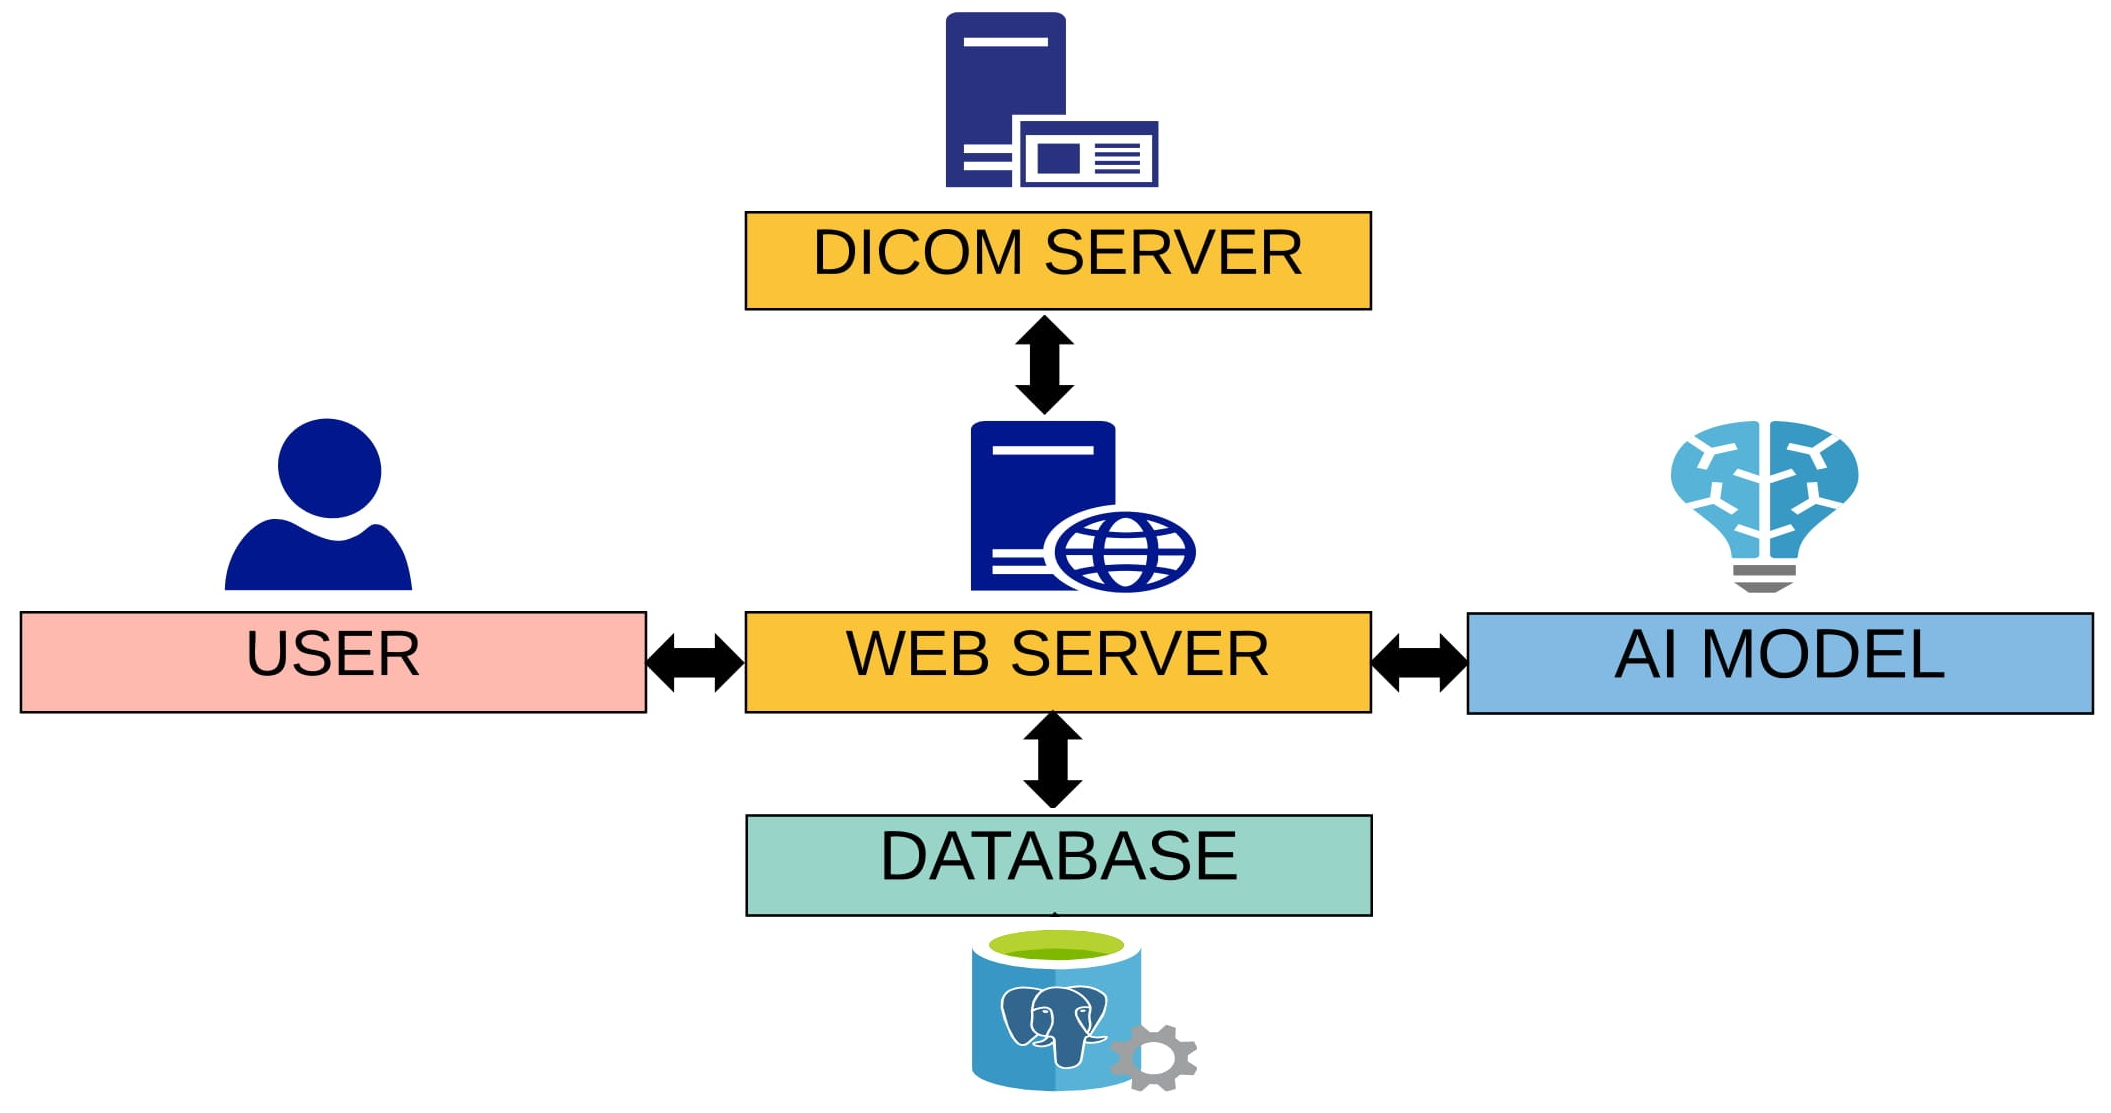
\includegraphics[width=14cm]{images/chapter-07-images/mvt-1.jpg}
    \caption{Tổng quan kiến trúc hệ thống DAT}
\end{figure}
Hệ thống DAT được xây dựng dựa trên mô hình MVT (Model - View - Template) của framework Django kết hợp với mô hình dự báo nhãn (AI MODEL).  

\begin{itemize}
    \item Model: Đây là phần trung gian chịu trách nhiệm xử lý dữ liệu giữa phần view (hiển thị cho người dùng) và phần cơ sở dữ liệu PostgreSQL. Model định nghĩa cấu trúc dữ liệu được lưu trữ cho phần dữ liệu đến từ View và truy xuât thông tin từ cơ sử dữ liệu, trả về cho View ở dạng xem được. Mỗi Model trong Django tương ứng với một bảng trong cơ sử dữ liệu. 
    \item View: Chịu trách nhiệm cho những gì người dùng thấy ở phía client. Một hàm view trong mô hình Django là một hàm Python nhận yêu cầu (“POST”,”GET”) từ phía người dùng và trả về một web response, response này có thể là nội dung HTML của trang web, một chuyển trang, một hình ảnh hoặc một response ở dạng JSON. 
    \item Template: Là phần thứ ba trong mô hình MVT, Template được viết bằng HTML, CSS và Javascript trong một file .html. Template cung cấp bố cục và giao diện trang web cho người dùng.
    \item Orthanc Server: Là nơi lưu trữ ảnh y khoa phục vụ việc lãm nhãn dữ liệu. 
    \item AI Model: Để việc làm nhãn được thuận tiện, nhanh chóng và chính xác hơn, AI Model được tích hợp vào hệ thống DAT. AI Model được chạy trong Django server và chịu trách nhiệm nhận yêu cầu từ phía client và trả về kết quả dự đoán. 
\end{itemize}

\subsection{Chi tiết kiến trúc hệ thống}
\subsubsection{Sơ đồ use case}
\begin{figure}[H]
    \centering
    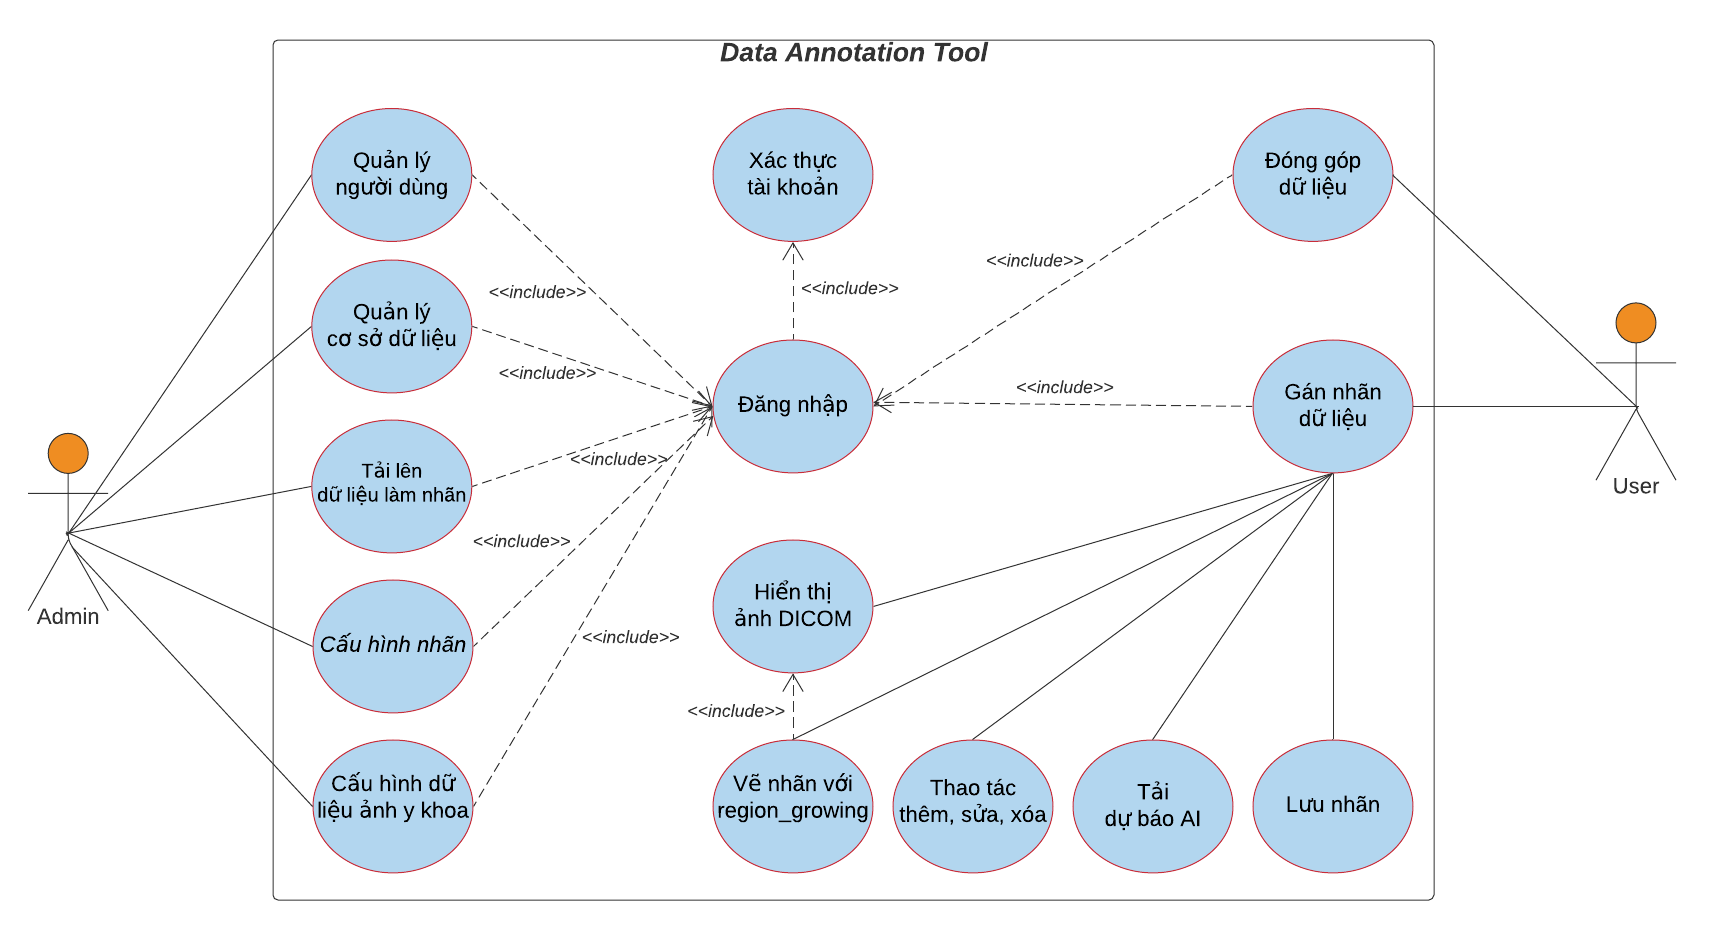
\includegraphics[width=14cm]{images/chapter-07-images/use-case-dat.png}
    \caption{Sơ đồ use case hệ thống DAT}
\end{figure}

\subsubsection{Sơ đồ sequence diagram}
\begin{figure}[H]
    \centering
    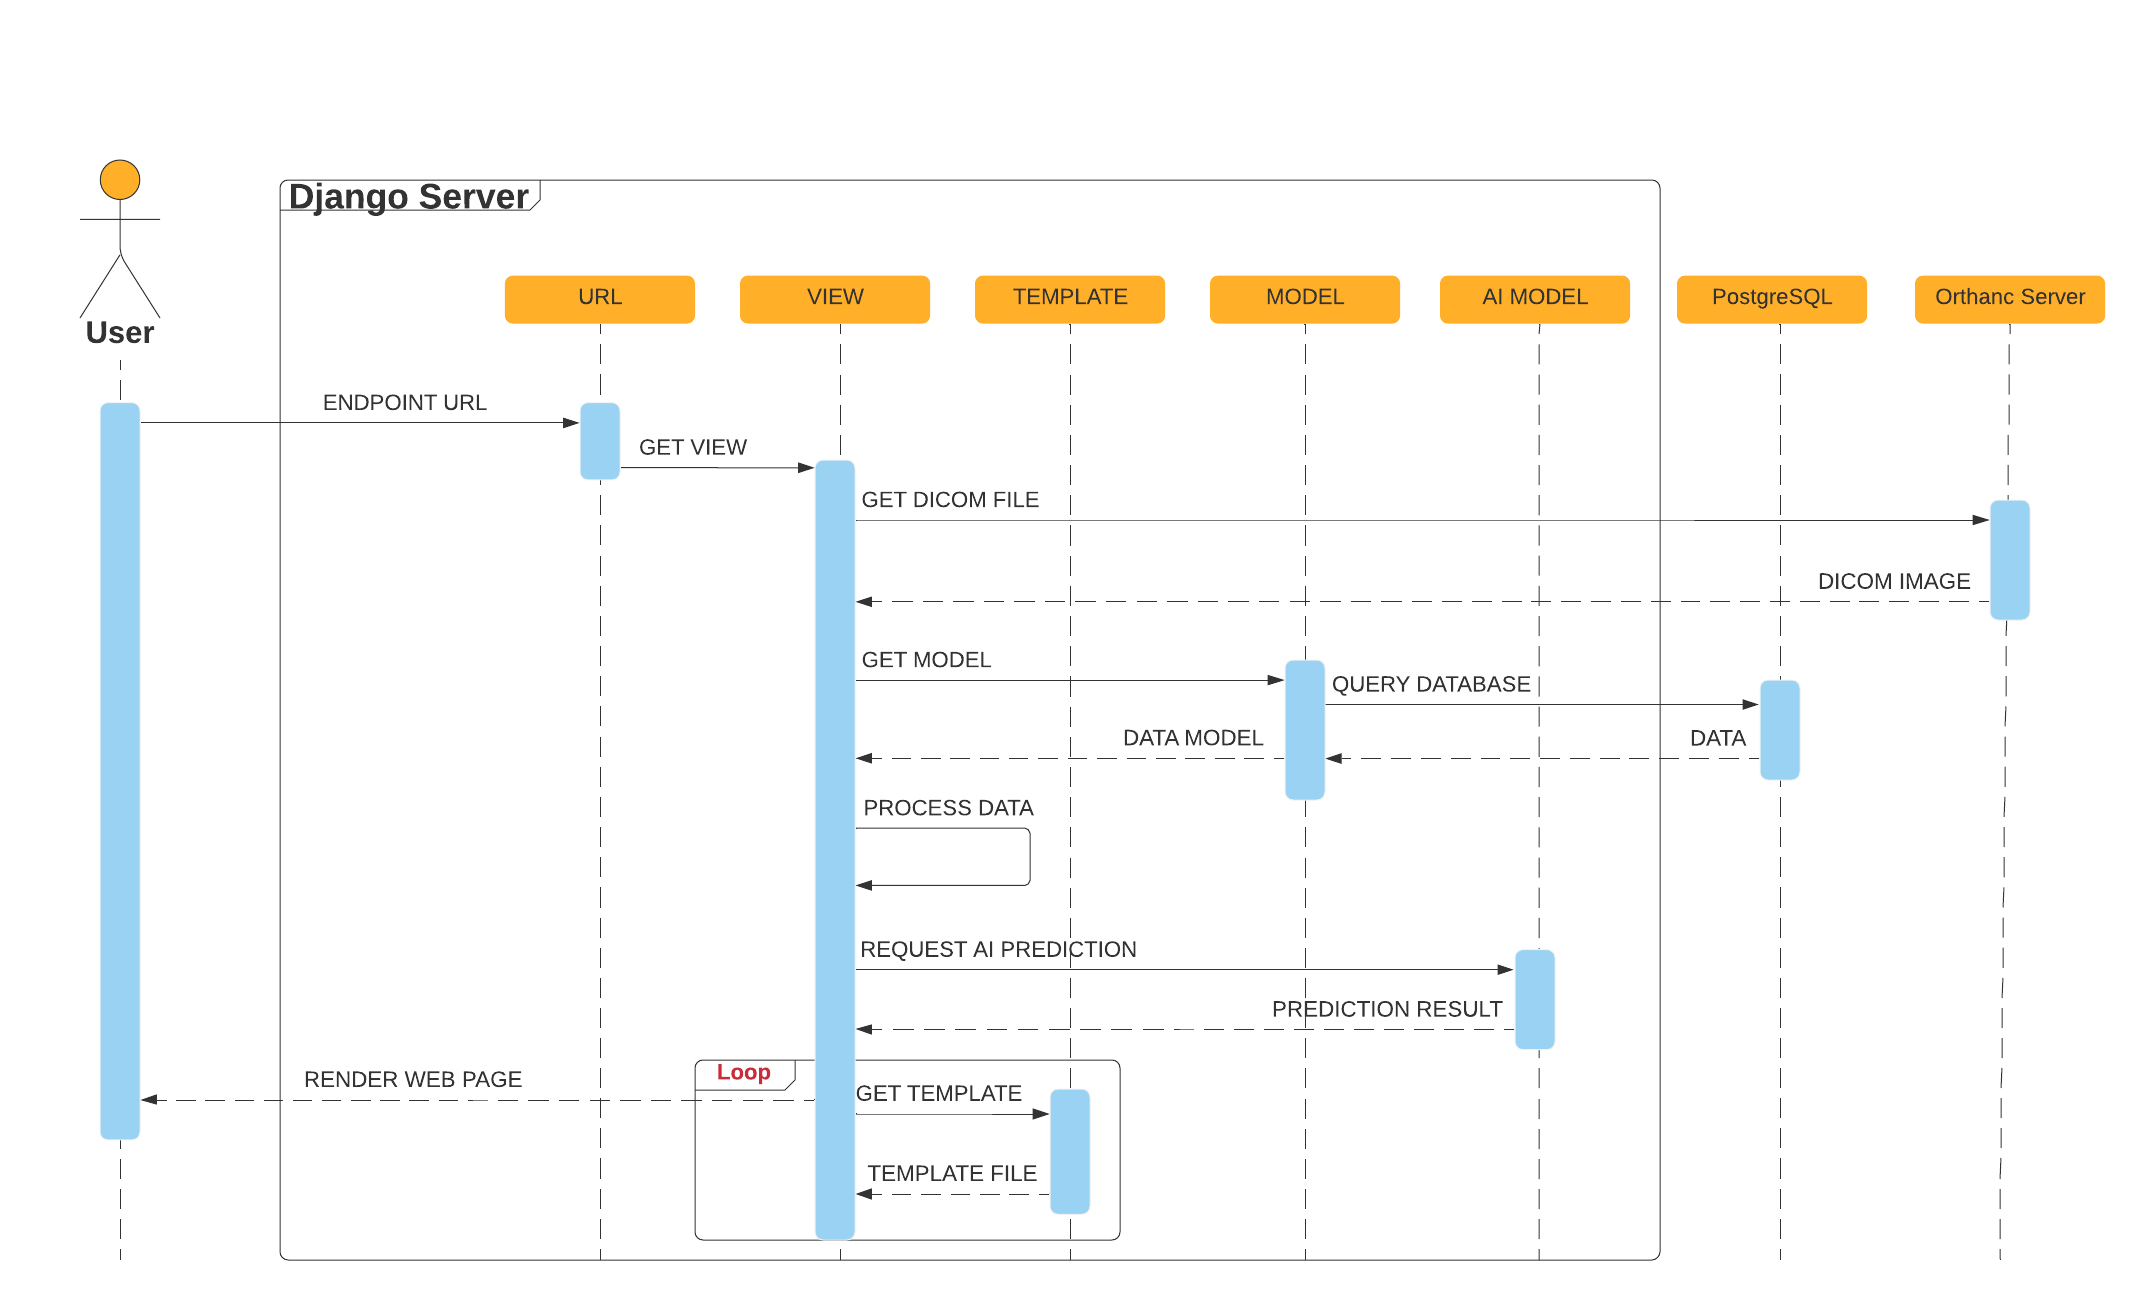
\includegraphics[width=14cm]{images/chapter-07-images/sequence-diagram.png}
    \caption{Sơ đồ sequence diagram hệ thống DAT}
\end{figure}

\subsubsection{Thiết kế cơ sở dữ liệu với Django Models}
Framework Django hỗ trợ lớp model để người dùng tương tác với cơ sở dữ liệu, mỗi model là một bảng gồm những trường được mô tả và quan hệ với các model khác (nếu có). Với hệ thống DAT này, ngoài những bảng dữ liệu được kế thừa, chúng tôi thiết kế thêm hai bảng dữ liệu chính:
\begin{itemize}
    \item Bảng dữ liệu để lưu nhãn đã làm: Sau khi bước làm nhãn kết thúc, dữ liệu nhãn sẽ được lưu trong bảng này, có thể xuất ra file .csv.
    \item Bảng dữ liệu để lưu nhãn được dự đoán bằng AI: Với một tập dữ liệu mới, người dùng có thể chạy dự đoán AI để hỗ trợ việc làm nhãn. Sau lần chạy dự đoán AI đầu tiên, phần nhãn được AI dự đoán sẽ được lưu vào bảng dữ liệu này để phục vụ việc làm nhãn. 
\end{itemize}


\begin{figure}[H]
    \centering
    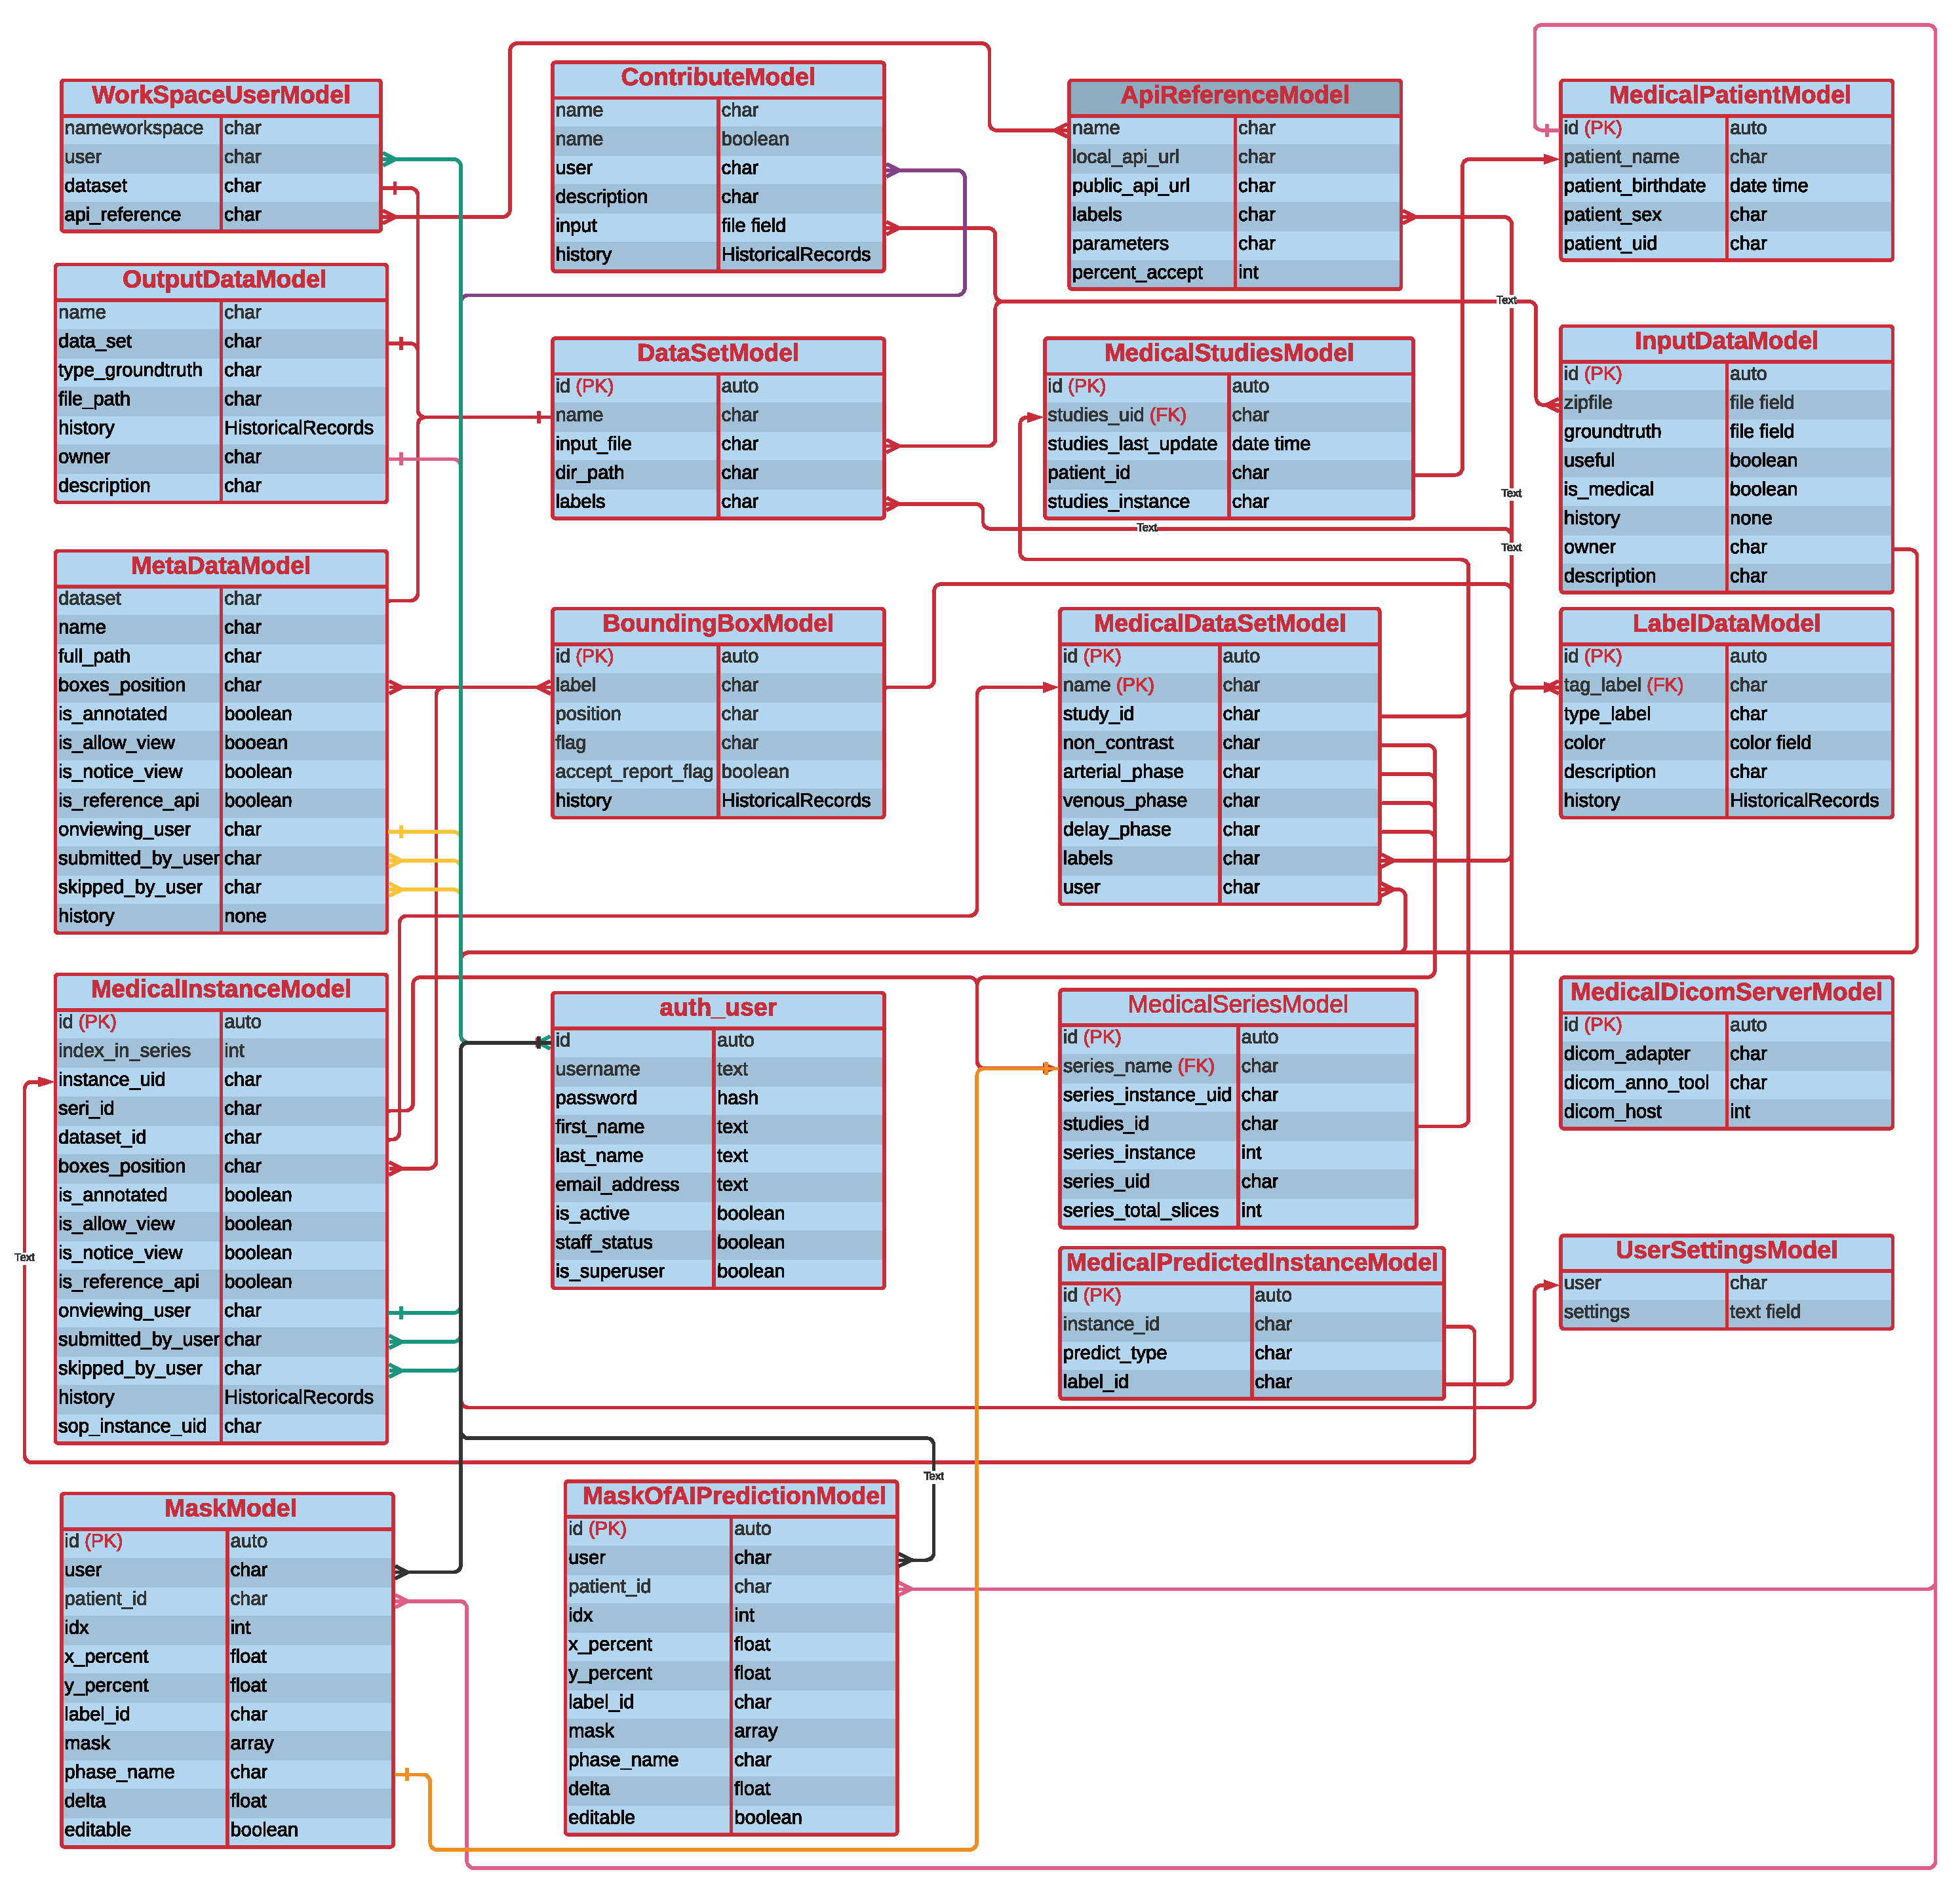
\includegraphics[width=17cm]{images/chapter-07-images/data-base-version-4.pdf}
    \caption{Thiết kế cơ sở dữ liệu với Django Model}
\end{figure}


\subsubsection{Cấu trúc mã nguồn hệ thống}
\begin{figure}[H]
    \centering
    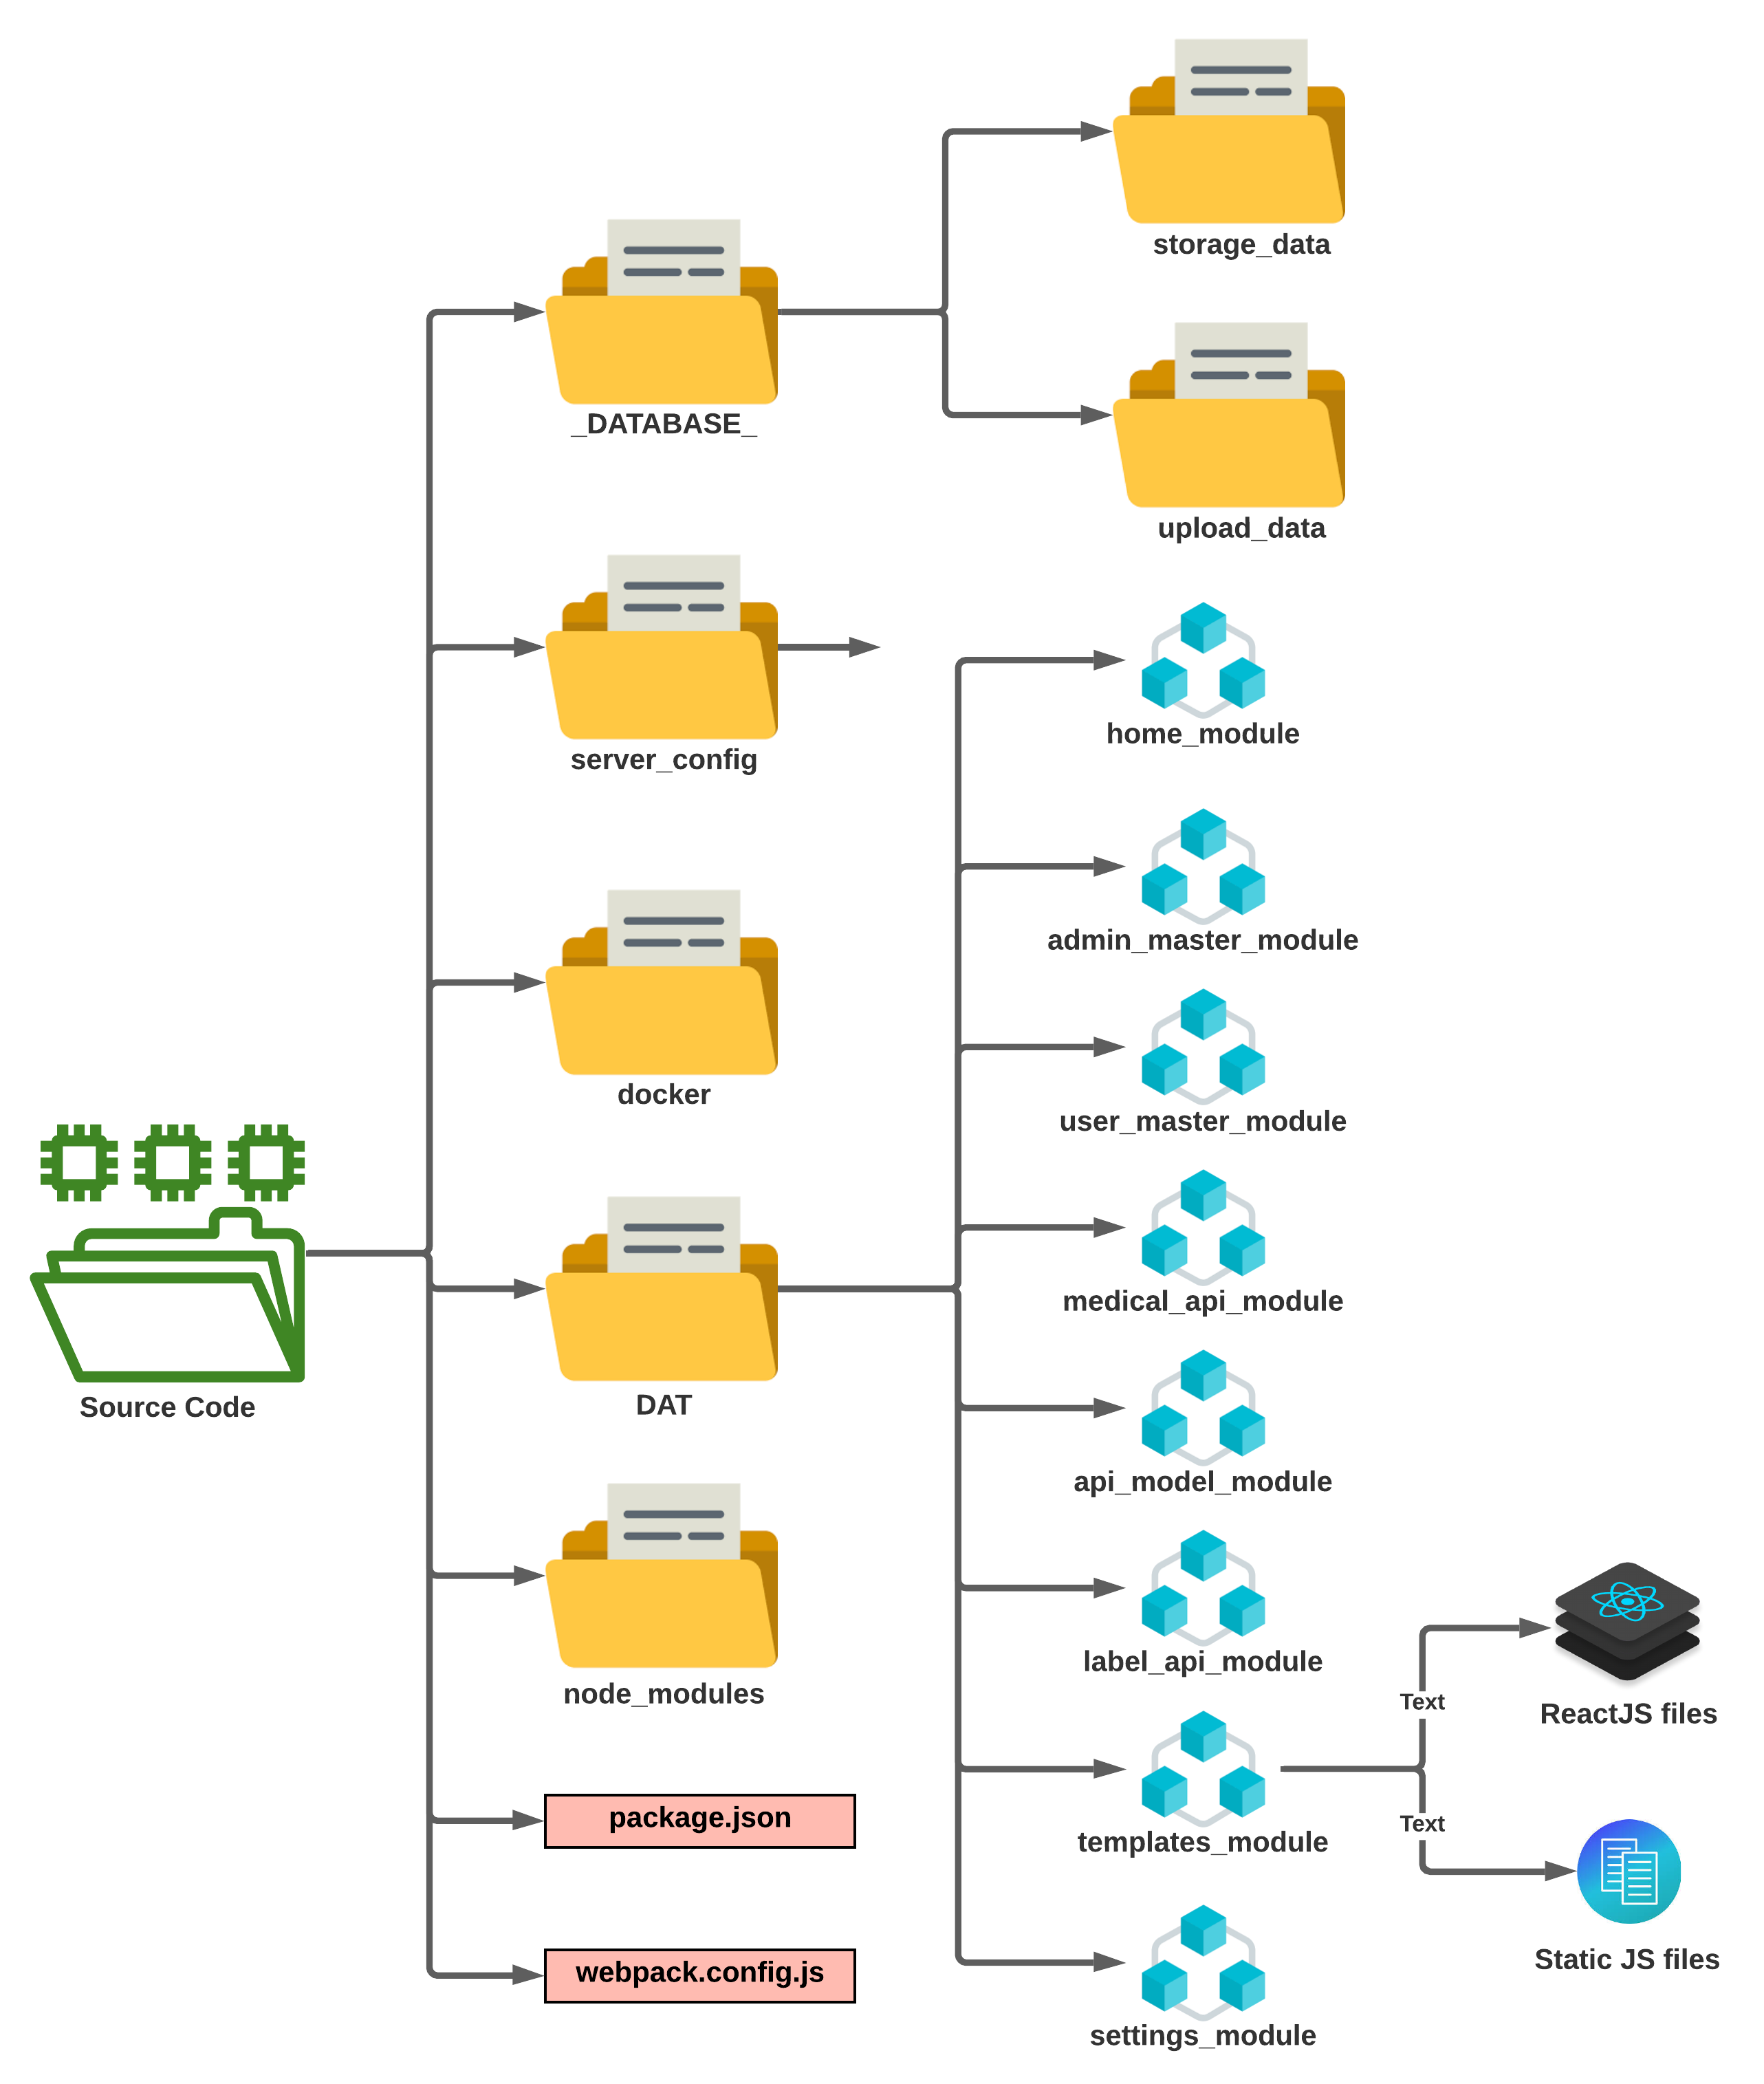
\includegraphics[width=14cm]{images/chapter-07-images/source-code-system.png}
    \caption{Cấu trúc mã nguồn hệ thống DAT}
\end{figure}


\section{Đặc tả tính năng hệ thống}
\newpage
\subsection{Tổng quan luồng hoạt động của hệ thống}
\begin{figure}[H]
    \centering
    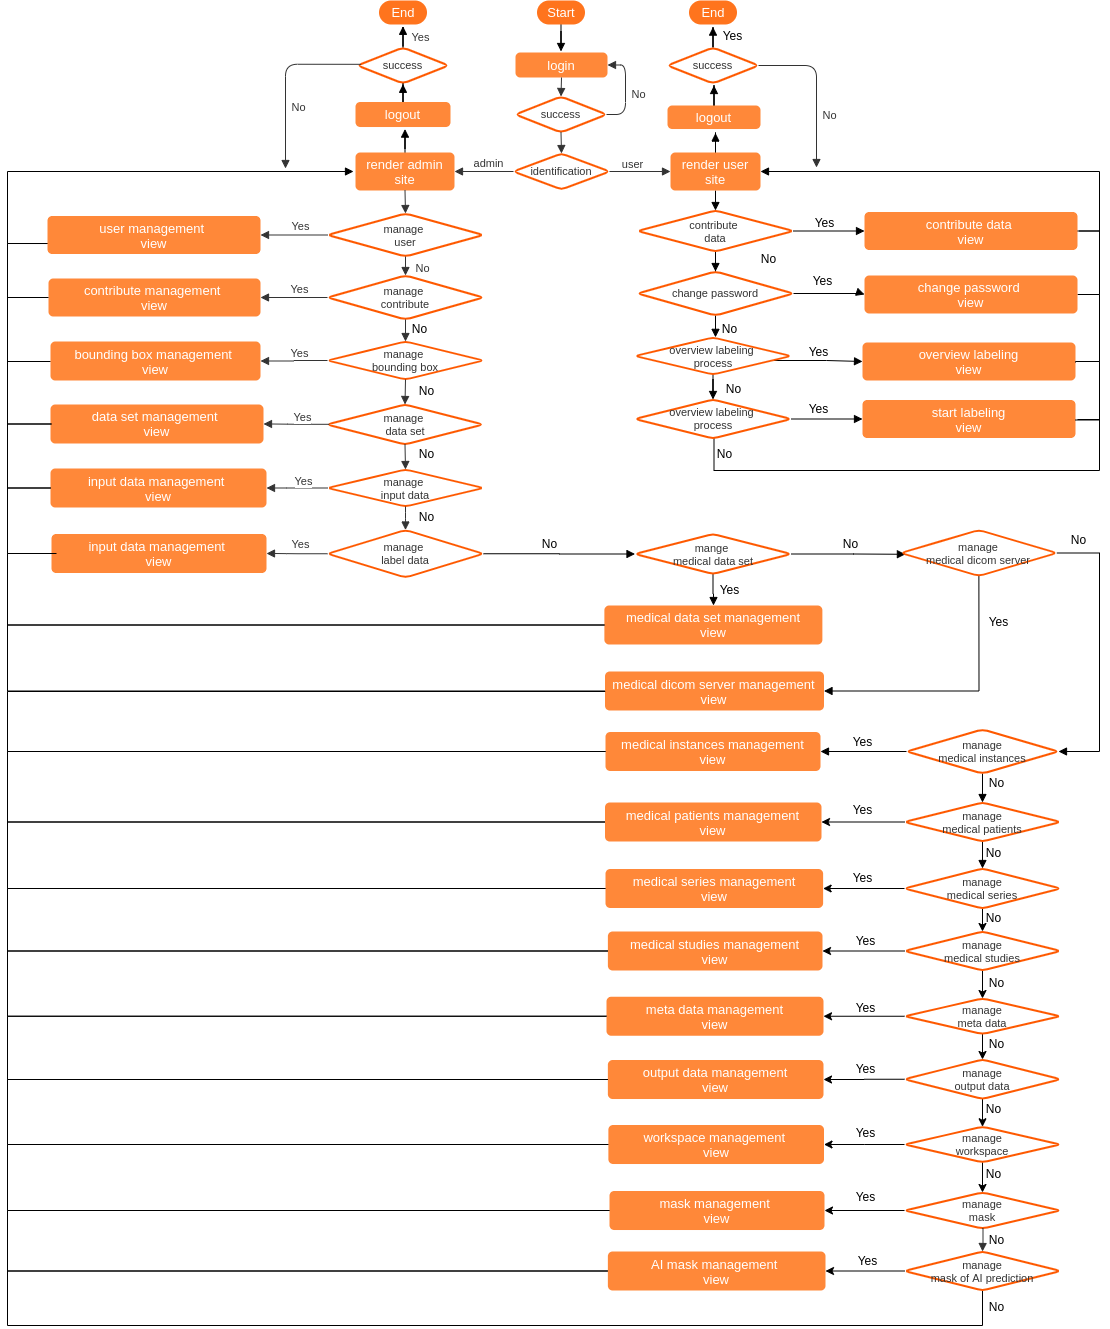
\includegraphics[width=16cm]{images/chapter-07-images/flow-chart-no-05.png}
    \caption{Luồng hoạt động hệ thống DAT}
\end{figure}


Flowchart với vai trò người quản trị

Flowchart với vai trò người dùng làm nhãn

\subsection{Chức năng đăng nhập và xác thực người dùng}
Hệ thống DAT hỗ trợ 2 vai trò đăng nhập khác nhau, một cho người quản trị hệ thống, hai cho người dùng làm nhãn. Với vai trò thứ nhất, sau khi đăng nhập thành công, người quản trị được phép thực hiện quản lý người dùng, quản lý dữ liệu làm nhãn, cấu hình nhãn và chỉ định người dùng lãm nhãn. Với vai trò thứ hai, sau khi đăng nhập, người dùng có thể  làm nhãn dữ liệu ảnh y khoa trên những tập dữ liệu đã được người quản trị chỉ định. 
\begin{figure}[H]
    \centering
    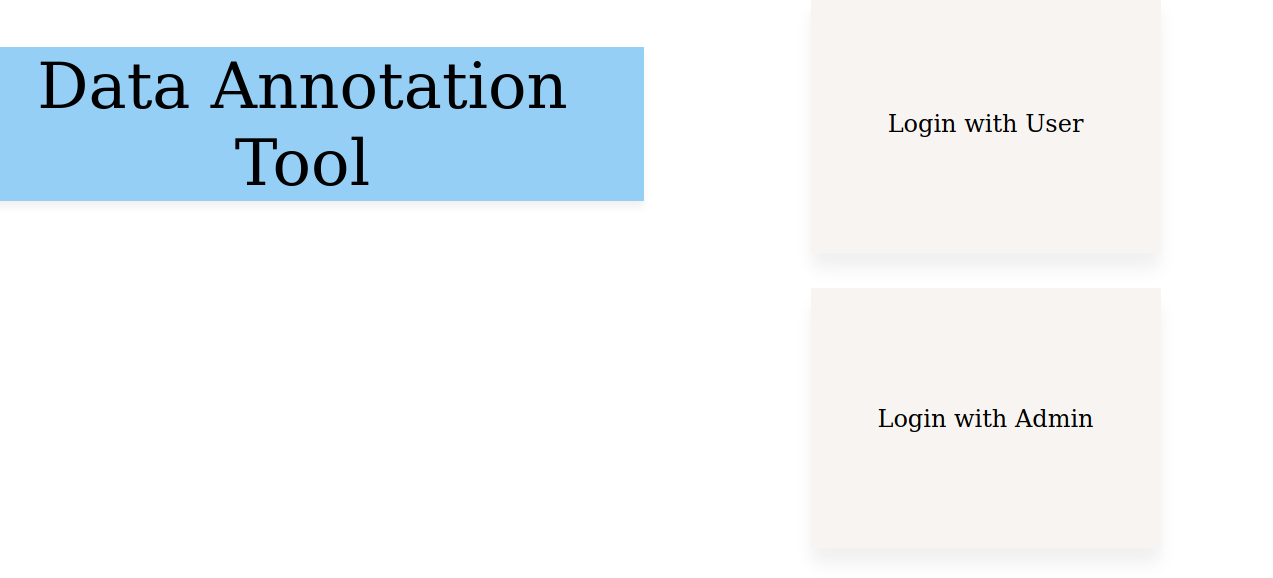
\includegraphics[width=14cm]{images/chapter-07-images/ui-dang-nhap.png}
    \caption{Giao diện đăng nhập của hệ thống DAT}
\end{figure}
\begin{figure}[H]
    \centering
    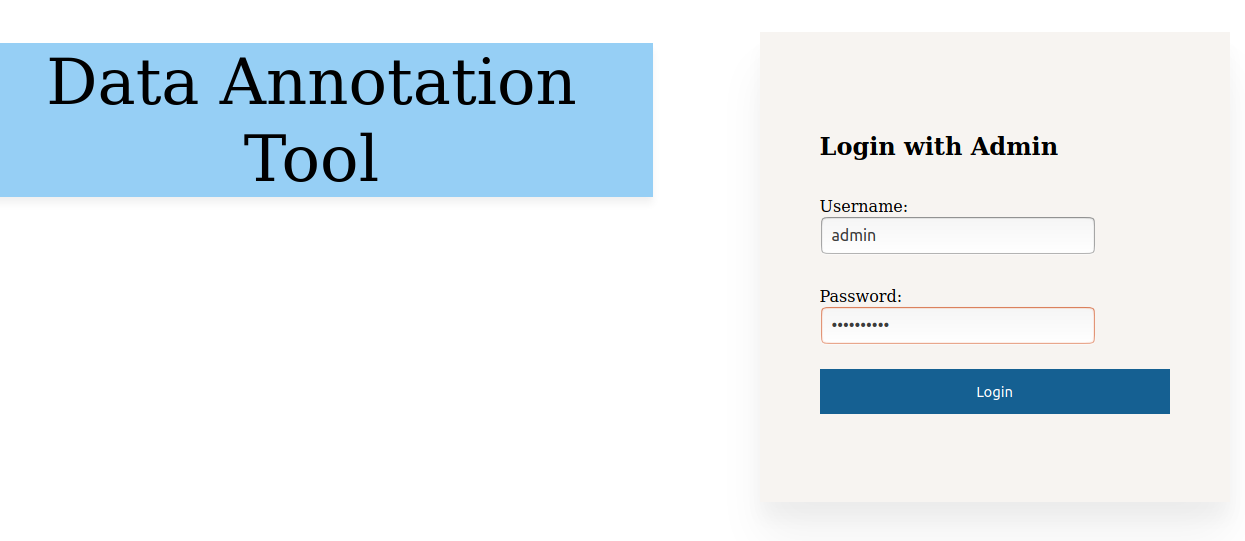
\includegraphics[width=14cm]{images/chapter-07-images/ui-dang-nhap-admin.png}
    \caption{Giao diện đăng nhập với vai trò admin của hệ thống DAT}
\end{figure}
\begin{figure}[H]
    \centering
    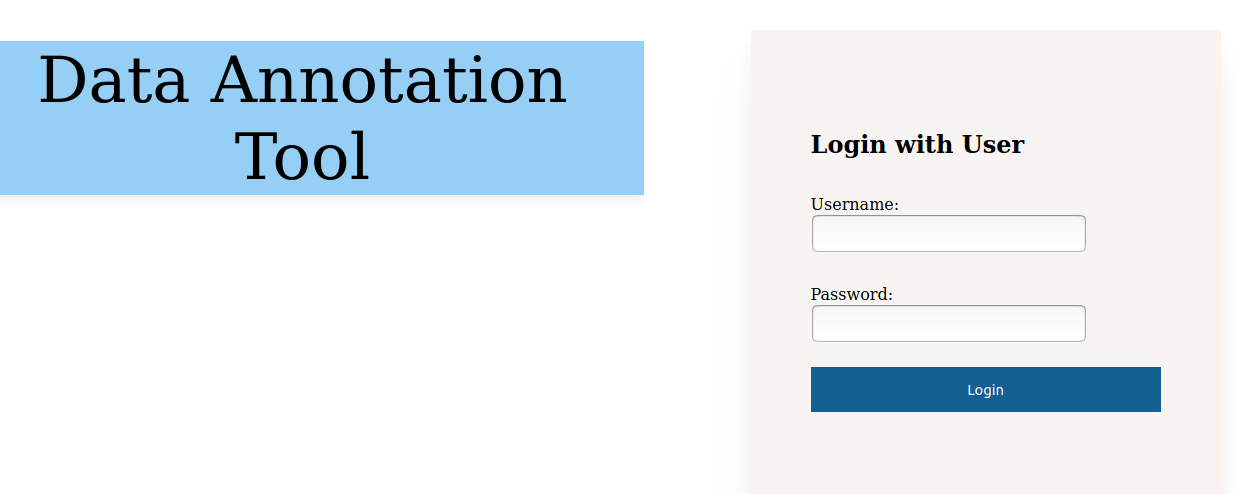
\includegraphics[width=14cm]{images/chapter-07-images/ui-dang-nhap-user.png}
    \caption{Giao diện đăng nhập với vai trò admin của hệ thống DAT}
\end{figure}

\subsection{Chức năng tải lên tập dữ liệu làm nhãn}
Hệ thống DAT cung cấp giao diện này để người quản trị tải lên tập dữ liệu ảnh y khoa cần làm nhãn. Tập tin được tải lên ở định dạng nén (.zip). Sau khi tải lên tập dữ liệu ảnh y khoa, người quản trị chọn mục "is medical image", đồng thời chỉ định chủ sở hữu dữ liệu và thêm phần mô tả ở bên dưới. Cuối cùng, người quản trị chọn lưu và có thể thoát hoặc tải lên tập dữ liệu khác.

\begin{figure}[H]
    \centering
    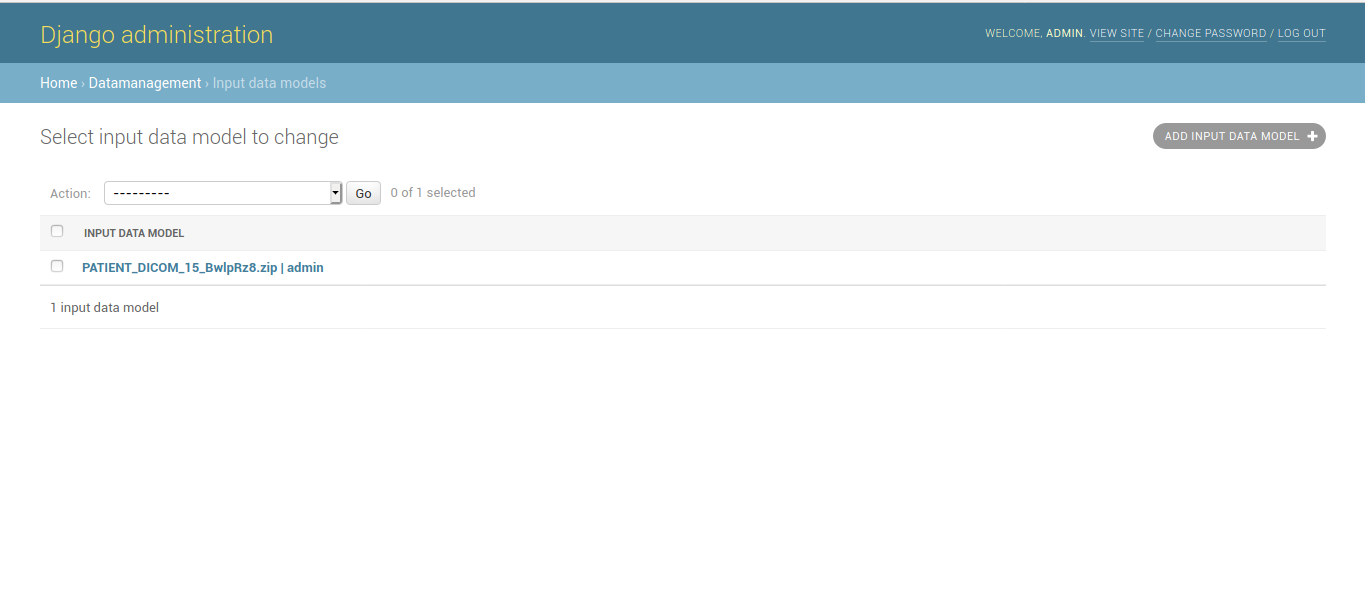
\includegraphics[width=14cm]{images/chapter-07-images/admin-input-data-model-1.png}
    \caption{Giao diện đăng nhập với vai trò admin của hệ thống DAT}
\end{figure}

\begin{figure}[H]
    \centering
    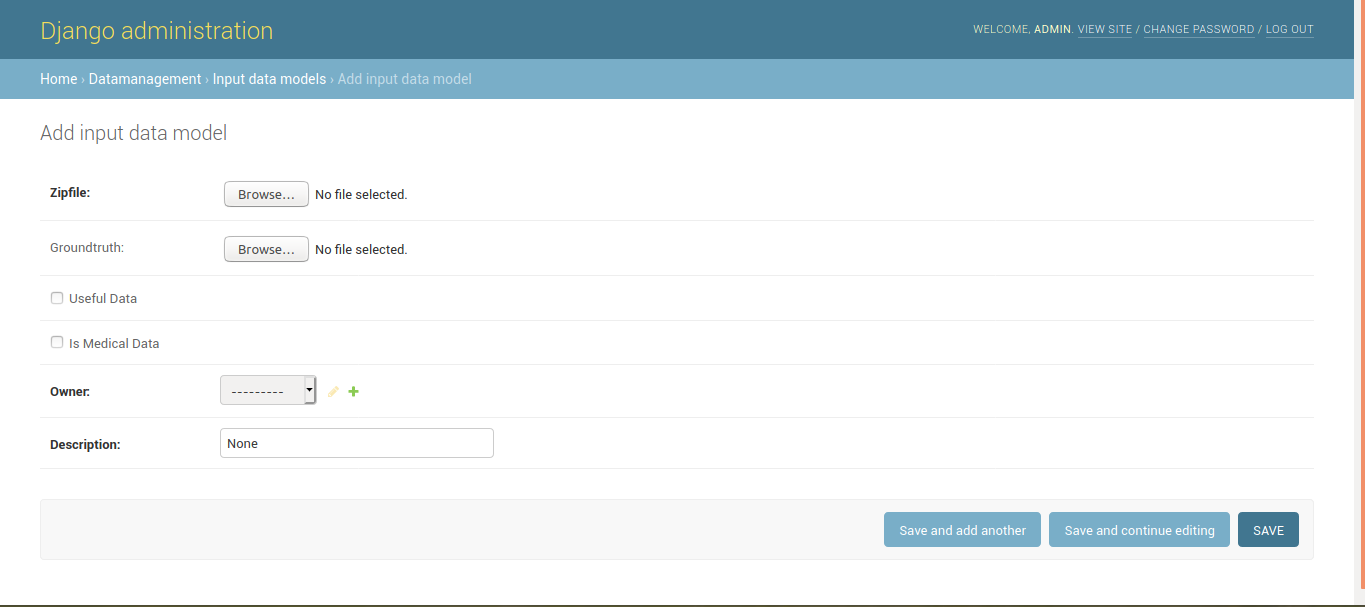
\includegraphics[width=14cm]{images/chapter-07-images/admin-input-data-model-2.png}
    \caption{Giao diện đăng nhập với vai trò admin của hệ thống DAT}
\end{figure}

\subsection{Chức năng cấu hình tập dữ liệu ảnh y khoa và chỉ định người lãm nhãn}
Để cấu hình tập dữ liệu ảnh y khoa, hệ thống DAT cung cấp mục \textbf{\textit{Medical data set model}}. Người quản trị bấm chọn tập dữ liệu cần cấu hình, sau đó chọn 4 thì tương ứng bao gồm: thì không thuốc, thì động mạch, thì tĩnh mạch và thì muộn. Tiếp tục chọn loại nhãn cần làm trên tập dữ liệu này, đồng thời chỉ định người làm nhãn và bấm nút lưu. 
\begin{figure}[H]
    \centering
    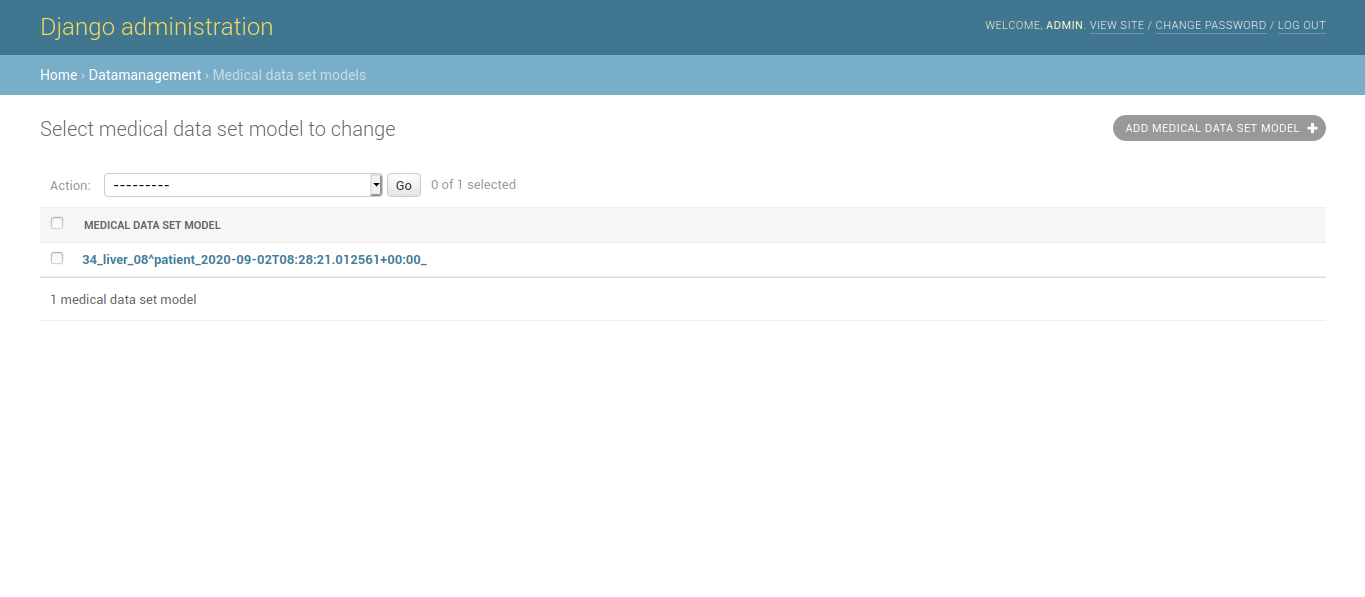
\includegraphics[width=14cm]{images/chapter-07-images/admin-medical-dataset-model-1.png}
    \caption{Giao diện đăng nhập với vai trò admin của hệ thống DAT}
\end{figure}
\begin{figure}[H]
    \centering
    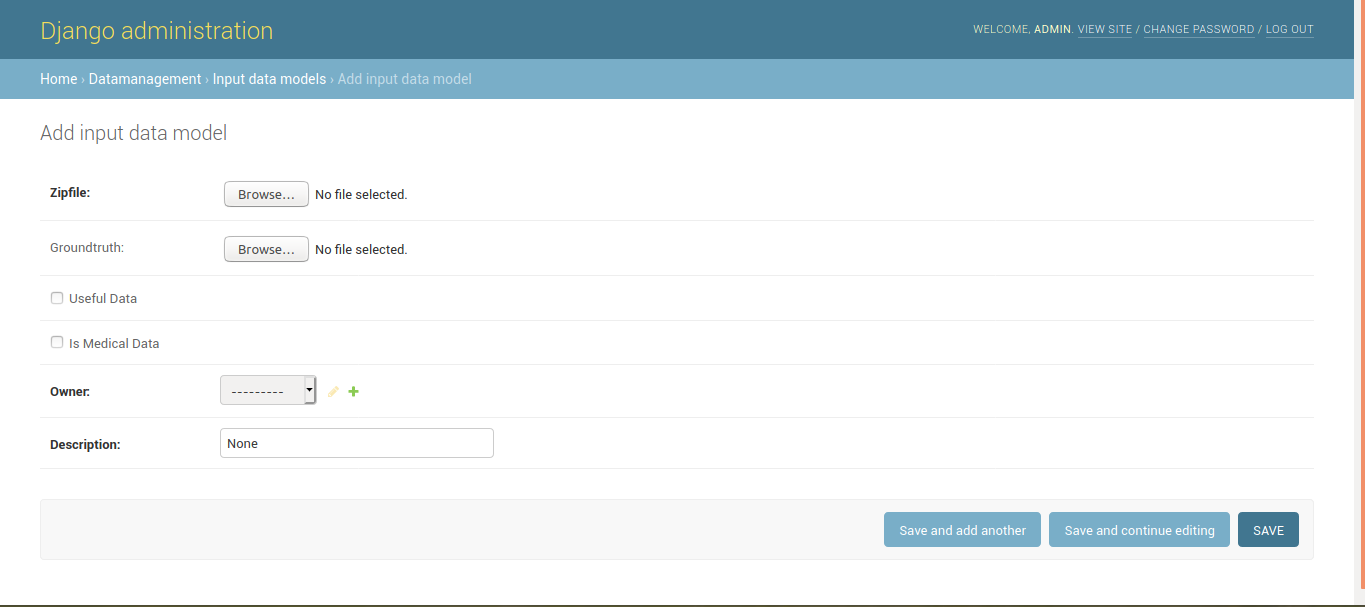
\includegraphics[width=14cm]{images/chapter-07-images/admin-input-data-model-2.png}
    \caption{Giao diện đăng nhập với vai trò admin của hệ thống DAT}
\end{figure}


\subsection{Chức năng làm nhãn dữ liệu y khoa}
Sau khi đăng nhập thành công, những tập dữ liệu nào đã được người quản trị chỉ định sẽ hiện trên giao diện chính của người dùng. Người dùng tiến hành bấm chọn tập dữ liệu cần thao tác và sau đó  bắt đầu làm nhãn. \\
\indent Hệ thống DAT hỗ  trợ dự đoán AI cho tập dữ liệu ảnh y khoa cần làm nhãn, giúp quá trình làm nhãn nhanh và tiện lợi hơn. Ngoài ra, hệt thống DAT còn hỗ trợ làm nhãn với giải thuật tăng trưởng vùng theo độ sáng, vẽ bằng bút, xóa, undo,...\\
\indent Phân giao diện chính với thanh menu bên trái và phần làm nhãn tương ứng với bốn thì (không thuốc, động mạch, tĩnh mạch và thì muộn) của ảnh DICOM bên phải. 

\begin{figure}[H]
    \centering
    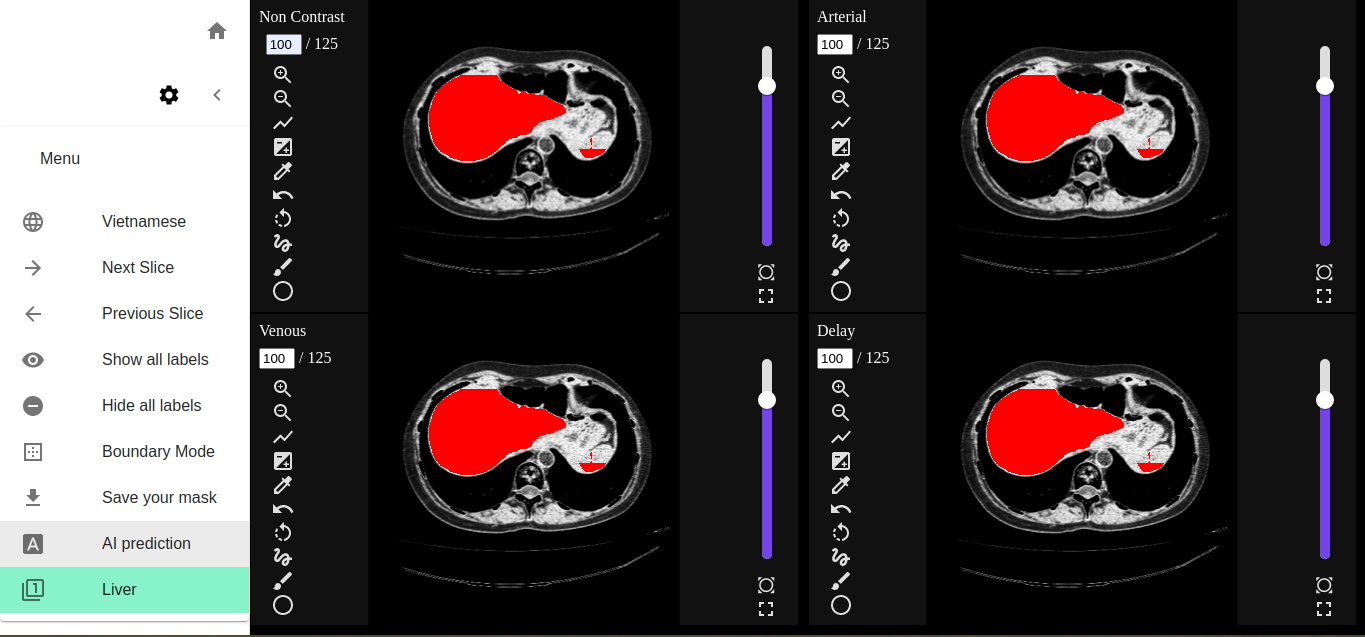
\includegraphics[width=\textwidth]{images/chapter-07-images/user-ui-medical-labeling.png}
    \caption{Tổng quan giao diện làm nhãn ảnh DICOM}
\end{figure}

\begin{figure}[H]
    \centering
    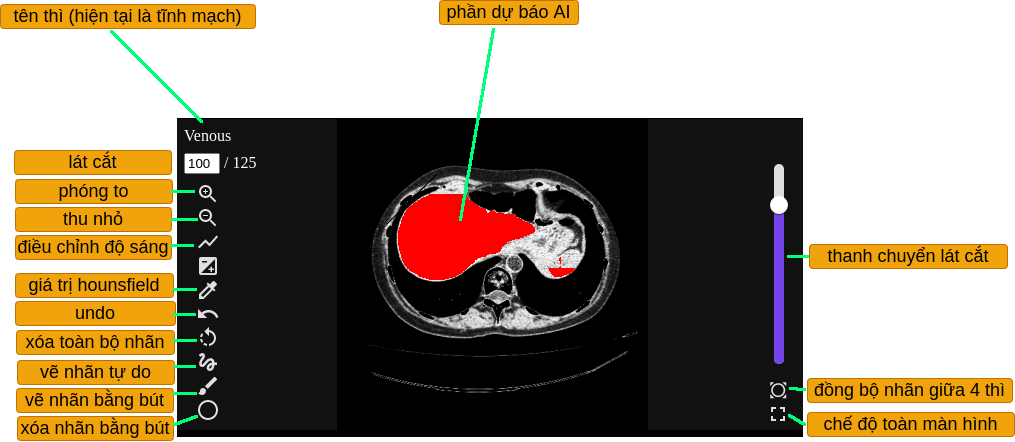
\includegraphics[width=\textwidth]{images/chapter-07-images/ui-labeling-13.png}
    \caption{Chi tiết giao diện làm nhãn ảnh DICOM}
\end{figure}

Để việc làm nhãn thuận lợi và nhanh chóng hơn, người dùng có thể chạy dự đoán AI (hiện lên nhãn màu đỏ).
\begin{figure}[H]
    \centering
    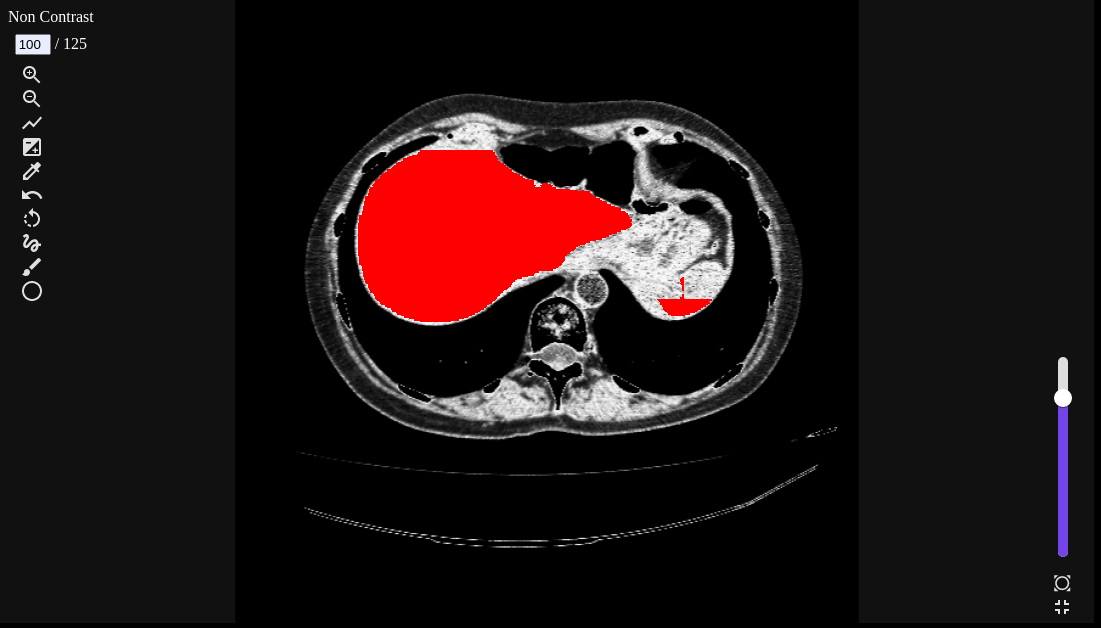
\includegraphics[width=\textwidth]{images/chapter-07-images/user-non-contrast-demo.png}
    \caption{Dự đoán AI cho phần làm nhãn ở thì không thuốc (Non contrast phase)}
\end{figure}

Để vẽ nhãn, người dùng có thể chọn chế  độ vẽ bằng bút, vẽ tự do hoặc vẽ với giải thuật tăng trưởng vùng theo mức sáng.
\begin{figure}[H]
    \centering
    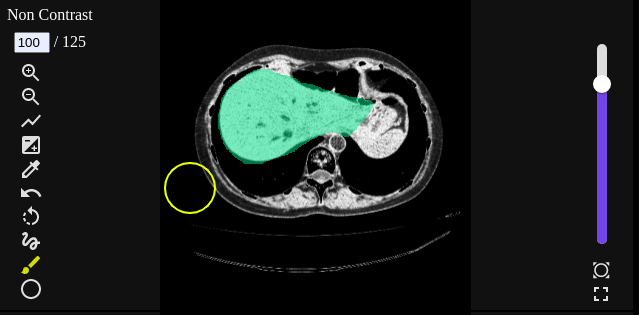
\includegraphics[width=\textwidth]{images/chapter-07-images/user-labeling-by-brush.png}
    \caption{Vẽ nhãn bằng bút trên ảnh DICOM ở thì không thuốc}
\end{figure}

\begin{figure}[H]
    \centering
    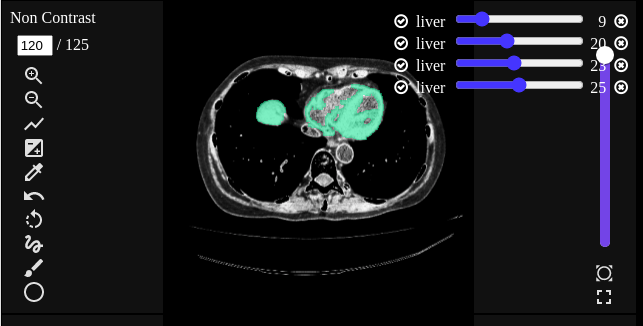
\includegraphics[width=\textwidth]{images/chapter-07-images/ui-labeling-region-growing.png}
    \caption{Vẽ nhãn với giải thuật tăng trưởng vùng trên ảnh DICOM ở thì không thuốc}
\end{figure}

\begin{figure}[H]
    \centering
    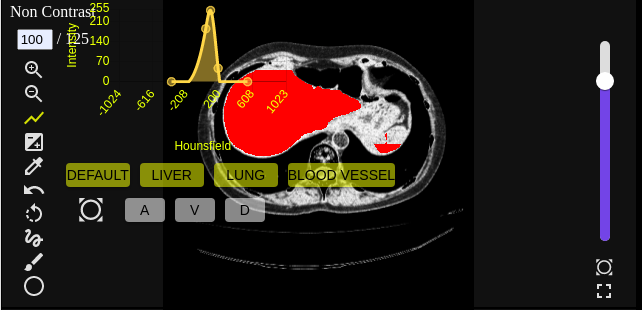
\includegraphics[width=\textwidth]{images/chapter-07-images/ui-adjust-contrast.png}
    \caption{Điểu chỉnh độ sáng để  làm nổi bật đối tượng cần làm nhãn}
\end{figure}

\begin{figure}[H]
    \centering
    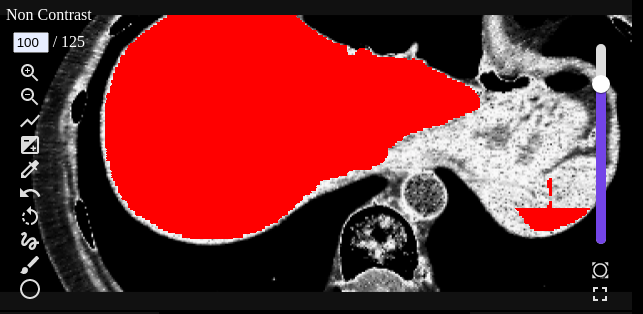
\includegraphics[width=\textwidth]{images/chapter-07-images/user-zoom-in.png}
    \caption{Phóng to một vùng trong ảnh DICOM}
\end{figure}


\section{Đánh giá và so sánh hệ thống DAT}
\subsection{Đánh giá hệ thống DAT}
\subsubsection{Ưu điểm}
\begin{itemize}
    \item Hỗ  trợ dự đoán AI vào phần ảnh DICOM cần làm nhãn, từ đó giảm thời gian làm nhãn đáng kể so với thông thường. Với những mô hình phân đoạn gan hiện tại, kết quả hệ số dice đều lớn hơn 90 phần trăm, vì vậy sau khi chạy dự đoán AI, người dùng chỉ cần thao tác rất ít để đạt được một nhãn chính xác.
    \item Giải thuật tăng trưởng vùng (region growing) theo độ sáng hỗ trợ làm nhãn nhanh, tiện lợi. 
    \item Có thể điều chỉnh độ sáng của ảnh để làm nổi bật  một số đối tượng cụ thể, ví dụ gan, mạch máu, phổi. 
    \item Cung cấp nhiều chế độ vẽ bao gồm vẽ nhãn bằng bút, vẽ nhãn bằng thao tác kéo thả chuột (free draw mode)
    \item Đồng bộ nhãn giữa 4 thì: thì không thuốc, thì động mạch, thì tĩnh mạch và thì muộn. 
    \item Hỗ trợ hai ngôn ngữ:  Tiếng Anh và tiếng Việt
    \item Có thể chuyển đổi giữa hai chế độ hiển thị nhãn: chế độ hiển thị vùng và chế độ hiển thị biên. 
    \item Có thể thực hiện thao tác quay về (undo) và xóa toàn bộ nhãn (reset to empty mask) nếu cần thiết. 
\end{itemize}

\subsubsection{Nhược điểm}
\begin{itemize}
    \item Hệ thống phản hồi chậm với các thao tác phòng to, thu nhỏ, kéo thả hình ảnh. Lý do: Một vùng cố định ROI (region of interest) sẽ được chọn để phóng to, thu nhỏ, kéo thả vì vậy sau mỗi lần thay đổi kích thước, hệ thống DAT sẽ tải và hiển thị lại vùng ROI này, dẫn đến việc UI phản hồi chậm. 
    \item Chưa thể tách riêng và thao tác độc lập trên  từng phần nhãn khi vẽ. 
\end{itemize}

\subsection{So sánh với hệ thống làm nhãn TrainingData.io}
TrainingData.io là công cụ làm nhãn ảnh y khoa được thành lập bởi một nhóm nhà phát triển giải pháp cho Visual AI có trụ sở tại San Francisco - Mỹ. \\

\begin{figure}[H]
    \centering
    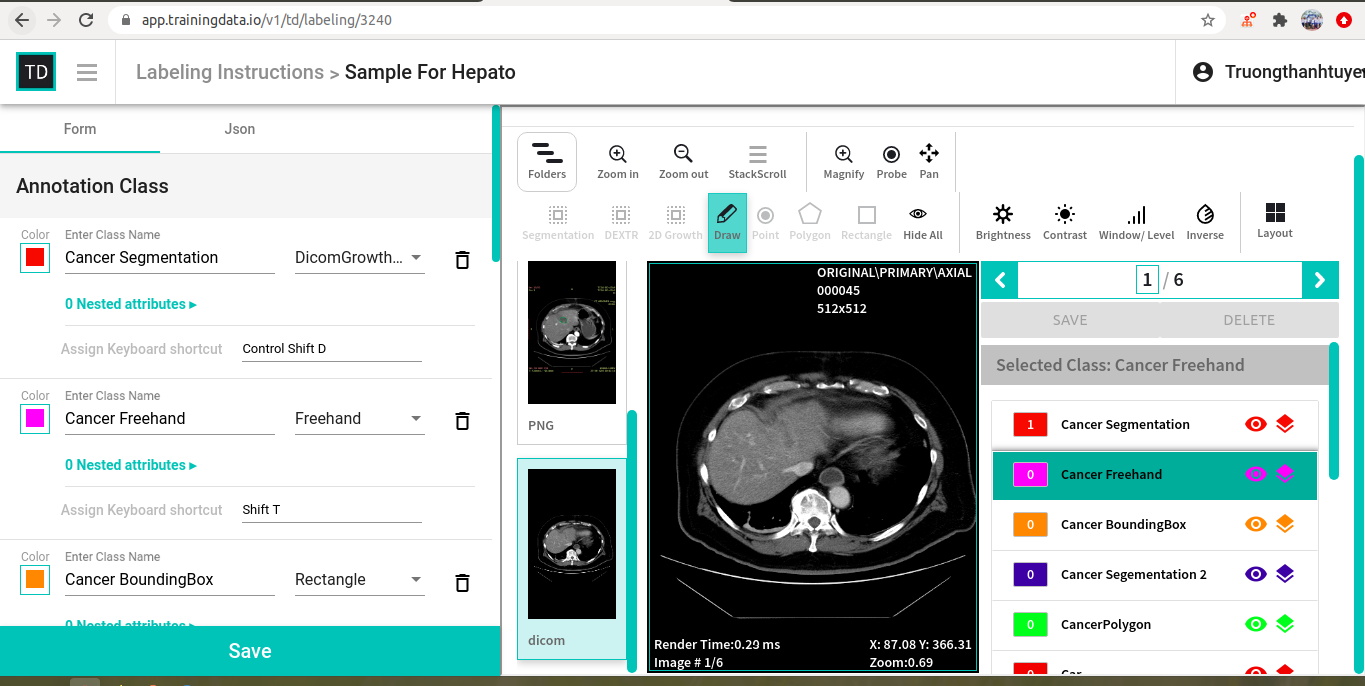
\includegraphics[width=\textwidth]{images/chapter-07-images/user-training-data-io.png}
    \caption{Công cụ làm nhãn TrainingData.io}
\end{figure}

\indent Nhóm chúng tôi xin phép so sánh phần làm nhãn dữ liệu ảnh DICOM giữa hệ thống DAT do nhóm thừa kế và phát triển với hệ thống TrainingData.io dựa trên một số tiêu chí cơ bản như sau: 

% begin table - comparison table
\begin{table}[H]
\begin{tabular}{|l|c|c|}
\hline
\multicolumn{1}{|c|}{\textbf{Tiêu chí so sánh}}                                                                                   & \textbf{Data Annotation Tool} & \textbf{TrainingData.io} \\ \hline
\begin{tabular}[c]{@{}l@{}}Tải lên tập dữ liệu cần \\ làm nhãn\end{tabular}                                                       & có                            & có                       \\ \hline
\begin{tabular}[c]{@{}l@{}}Quản lý người dùng \\ làm nhãn\end{tabular}                                                            & có                            & có                       \\ \hline
Cấu hình nhãn                                                                                                                     & có                            & có                       \\ \hline
Dự đoán AI                                                                                                                        & có                            & có                       \\ \hline
\begin{tabular}[c]{@{}l@{}}Vẽ nhãn với giải thuật \\ tăng trường vùng\end{tabular}                                                & có                            & có                    \\ \hline
\begin{tabular}[c]{@{}l@{}}Phóng to, thu nhỏ, \\ kéo thả nhanh\end{tabular}                                                       & chậm                          & nhanh                    \\ \hline
\begin{tabular}[c]{@{}l@{}}Tách riêng và thao tác \\ độc lập trên từng phần \\ nhãn\end{tabular}                                  & không                         & có                       \\ \hline
\begin{tabular}[c]{@{}l@{}}Vẽ nhãn tự do với \\ chuột  (dạng đa giác)\end{tabular}                                                & có                            & có                       \\ \hline
Vẽ nhãn bằng bút vẽ                                                                                                               & có                            & không                    \\ \hline
\begin{tabular}[c]{@{}l@{}}Hỗ trợ tiếng Việt và \\ tiếng Anh\end{tabular}                                                         & có                            & chỉ hỗ trợ tiếng Anh     \\ \hline
\begin{tabular}[c]{@{}l@{}}Tùy chỉnh độ sáng để \\ làm nổi  bật một số đối \\ tượng  cụ thể (gan, mạch\\  máu, phổi)\end{tabular} & có                            & không                    \\ \hline
\end{tabular}
\caption{So sánh hệ thống DAT và hệ thống TrainingData.io}
\end{table}
% end table - comparison table 


\subsection{Hướng phát triển hệ thống trong tương lai}
Tử việc so sánh với một số công cụ làm nhãn ảnh y khoa hiện có (ví dụ TrainingData.io), nhóm nhận thấy hệ thống DAT do nhóm kế thừa và phát triển cần cải thiện những điểm sau đây:
\begin{itemize}
    \item Thêm tính năng tách riêng và thao tác độc lập trên từng phần nhãn.
    \item Cải thiện phần tải và hiển thị ảnh DICOM, phần phóng to, thu nhỏ, kéo thả hình ảnh được nhanh hơn, tăng trải nghiệm người dùng. 
    \item Cần cải thiện giao diện làm nhãn vì  giao diện hiện tại còn tối, chưa bắt mắt, khó sử dụng cho người mới. 
\end{itemize}
% \section{Quy trình làm nhãn để xuất}

\section{Đóng góp}
Nhóm thừa kế những chức năng sau đây từ hệ thống làm nhãn DAT của phòng lab: 
\begin{itemize}[noitemsep]
    \item Chức năng đăng nhập và xác thực người dùng.
    \item Chức năng tải lên tập dữ liệu làm nhãn.
	\item Chức năng cấu hình tập dữ liệu ảnh y khoa và chỉ định người dùng làm nhãn.
	\item Chức năng hiện và ẩn nhãn.
	\item Chức năng hiển thị đường biên.
	\item Chức năng lấy ngưỡng giá trị Hounsfield để làm rõ đối tượng cần làm nhãn.
	\item Chức năng vẽ bằng bút.
	\item Chức năng xóa bằng bút.
	\item Chức năng chọn vùng ROI (region of interest).
\end{itemize}

Ngoài những chức năng được kế thừa từ hệ thống DAT của phòng lab Computer Vision and Graphics, nhóm chúng tôi đã cải thiện và phát triển mới những tính năng sau đây:
\begin{itemize}[noitemsep]
    \item Cải thiện tính năng làm nhãn với giải thuật tăng trưởng vùng theo mức xám.
    \item Tạo mới chức năng tích hợp dự đoán AI phục vụ việc làm nhãn.
    \item Tạo mới chức năng quay về (undo).
    \item Tạo mới chức năng xóa tòan bộ nhãn.
    \item Tạo mới chức năng vẽ nhãn tự do (dạng polygon).
    \item Tạo mới chức năng lưu nhãn đã làm.
    \item Tạo mới chức năng hỗ trợ ngôn ngữ tiếng Việt và tiếng Anh.
    \item Tạo mới chức năng phóng to, thu nhỏ, kéo thả hình ảnh khi làm nhãn.
    \item Tạo mới chức năng đồng bộ nhãn giữa 4 thì (thì không thuốc, thì động mạch, thì tĩnh mạch, thì muộn).
    \item Tạo mới thanh cuộn để chuyển giữa các lát cắt trong quá trình làm nhãn.
\end{itemize}




% https://topdev.vn/blog/webpack-la-gi/
% https://webpack.js.org/concepts/
% https://www.hostinger.vn/huong-dan/nginx-la-gi-no-hoat-dong-nhu-the-nao/
% https://medium.com/@phamducquan/docker-l%C3%A0-g%C3%AC-ki%E1%BA%BFn-th%E1%BB%A9c-c%C6%A1-b%E1%BA%A3n-v%E1%BB%81-docker-13c6efc4aefe
% https://medium.com/@jaychaturvedi18/a-brief-introduction-to-django-mvt-framework-8ef46cc321ab
% https://www.orthanc-server.com/static.php?page=about
% https://skillcrush.com/blog/what-is-react-js/
% https://viblo.asia/p/reactjs-uu-diem-va-nhuoc-diem-V3m5WzexlO7
% https://bizflycloud.vn/tin-tuc/postgresql-la-gi-tim-hieu-ve-co-so-du-lieu-ma-nguon-mo-tien-tien-nhat-the-gioi-20180919175924611.htm
% https://vinasupport.com/database/postgresql/
% https://thinhnotes.com/chuyen-nghe-ba/use-case-diagram-va-5-sai-lam-thuong-gap/
% 